\documentclass{beamer}
\usepackage[utf8]{inputenc}
\usepackage[slovene,english]{babel}
\usepackage{verbatim}

\usetheme{default}

\title{Vrtače Dinarskega krasa}

% A subtitle is optional and this may be deleted
% \subtitle{Optional Subtitle}

\author{Rok Mihevc \\ Mentor: prof. Rudolf Podgornik}

\institute[Univerza v Ljubljani]
{
\begin{center} 
  
\includegraphics[width=0.4\textwidth]{slike/logo_fmf_uni-lj_sl.pdf} 
\end{center}
}

\date{Ljubljana, 2014}


% Delete this, if you do not want the table of contents to pop up at
% the beginning of each subsection:
%\AtBeginSubsection[]
%{
%  \begin{frame}<beamer>{Outline}
%    \tableofcontents[currentsection,currentsubsection]
%  \end{frame}
%}


\begin{document}

\begin{frame}
  \titlepage
\end{frame}

\begin{frame}{Pregled}
  \tableofcontents
  % You might wish to add the option [pausesections]
\end{frame}


\section{Preučevanje realnih vrtač}

\subsection{Kraške vrtače}

\begin{frame}{Kraške vrtače}{So zaobljene lijakaste globeli}
\begin{center} 
  \hspace*{-0.075\textwidth}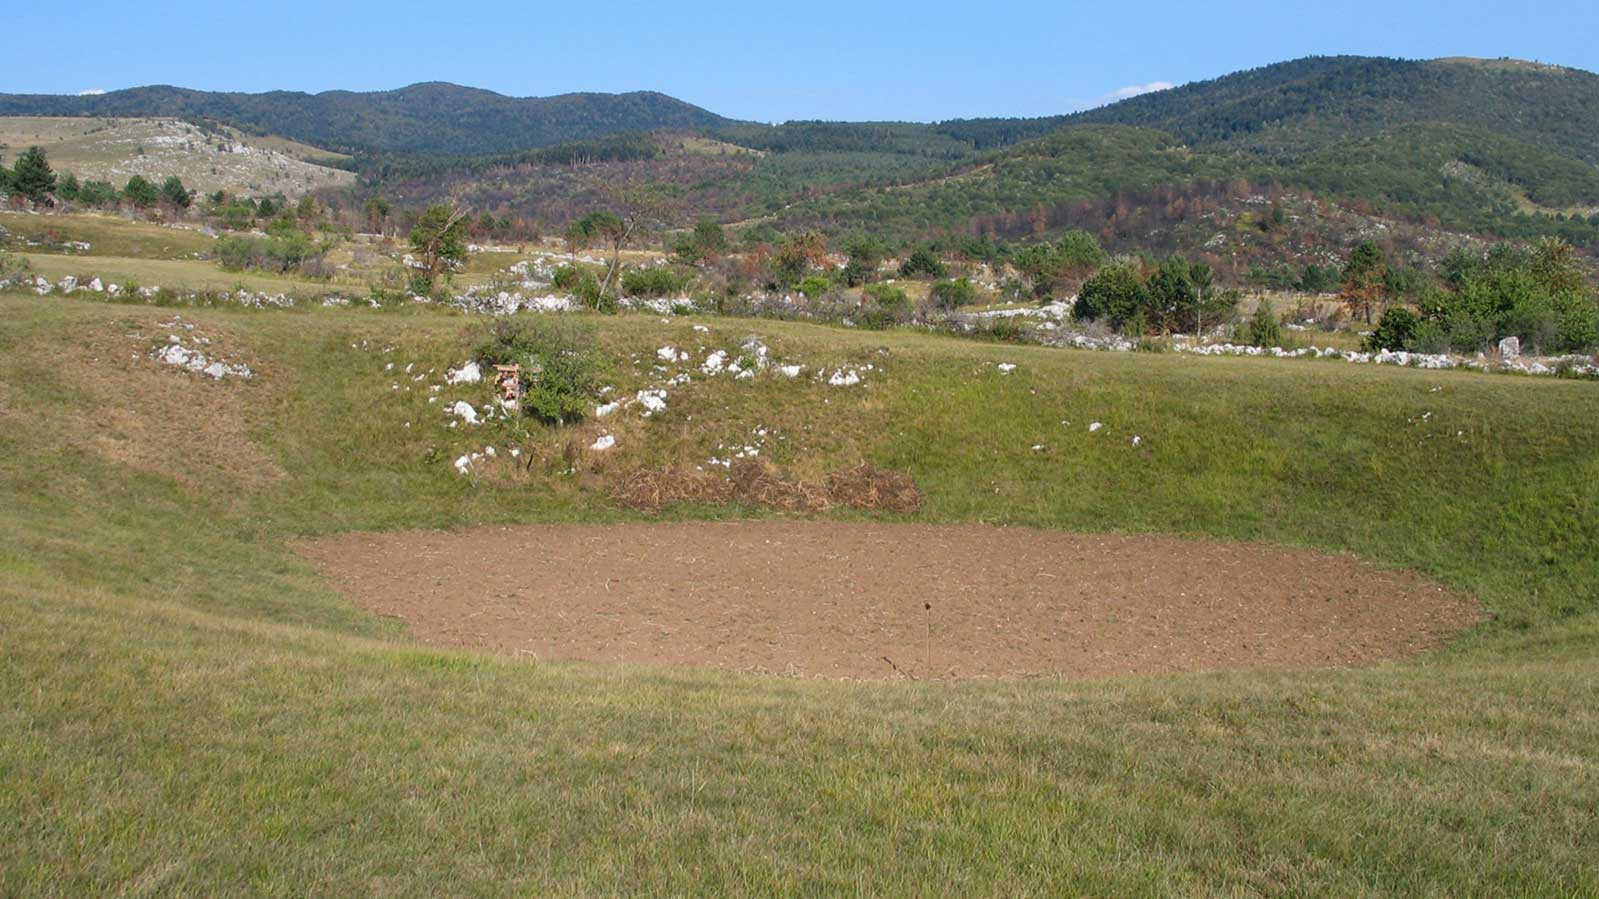
\includegraphics[width=1.15\textwidth]{slike/vrtaca} \\
  Jurišče, Slovenija \small{(vir: A.M.)}
\end{center} 
\end{frame}

\begin{frame}{Kraške vrtače}{Najdemo jih na starih kraških poljih in planotah}
  \begin{center}
    \hspace*{-0.075\textwidth}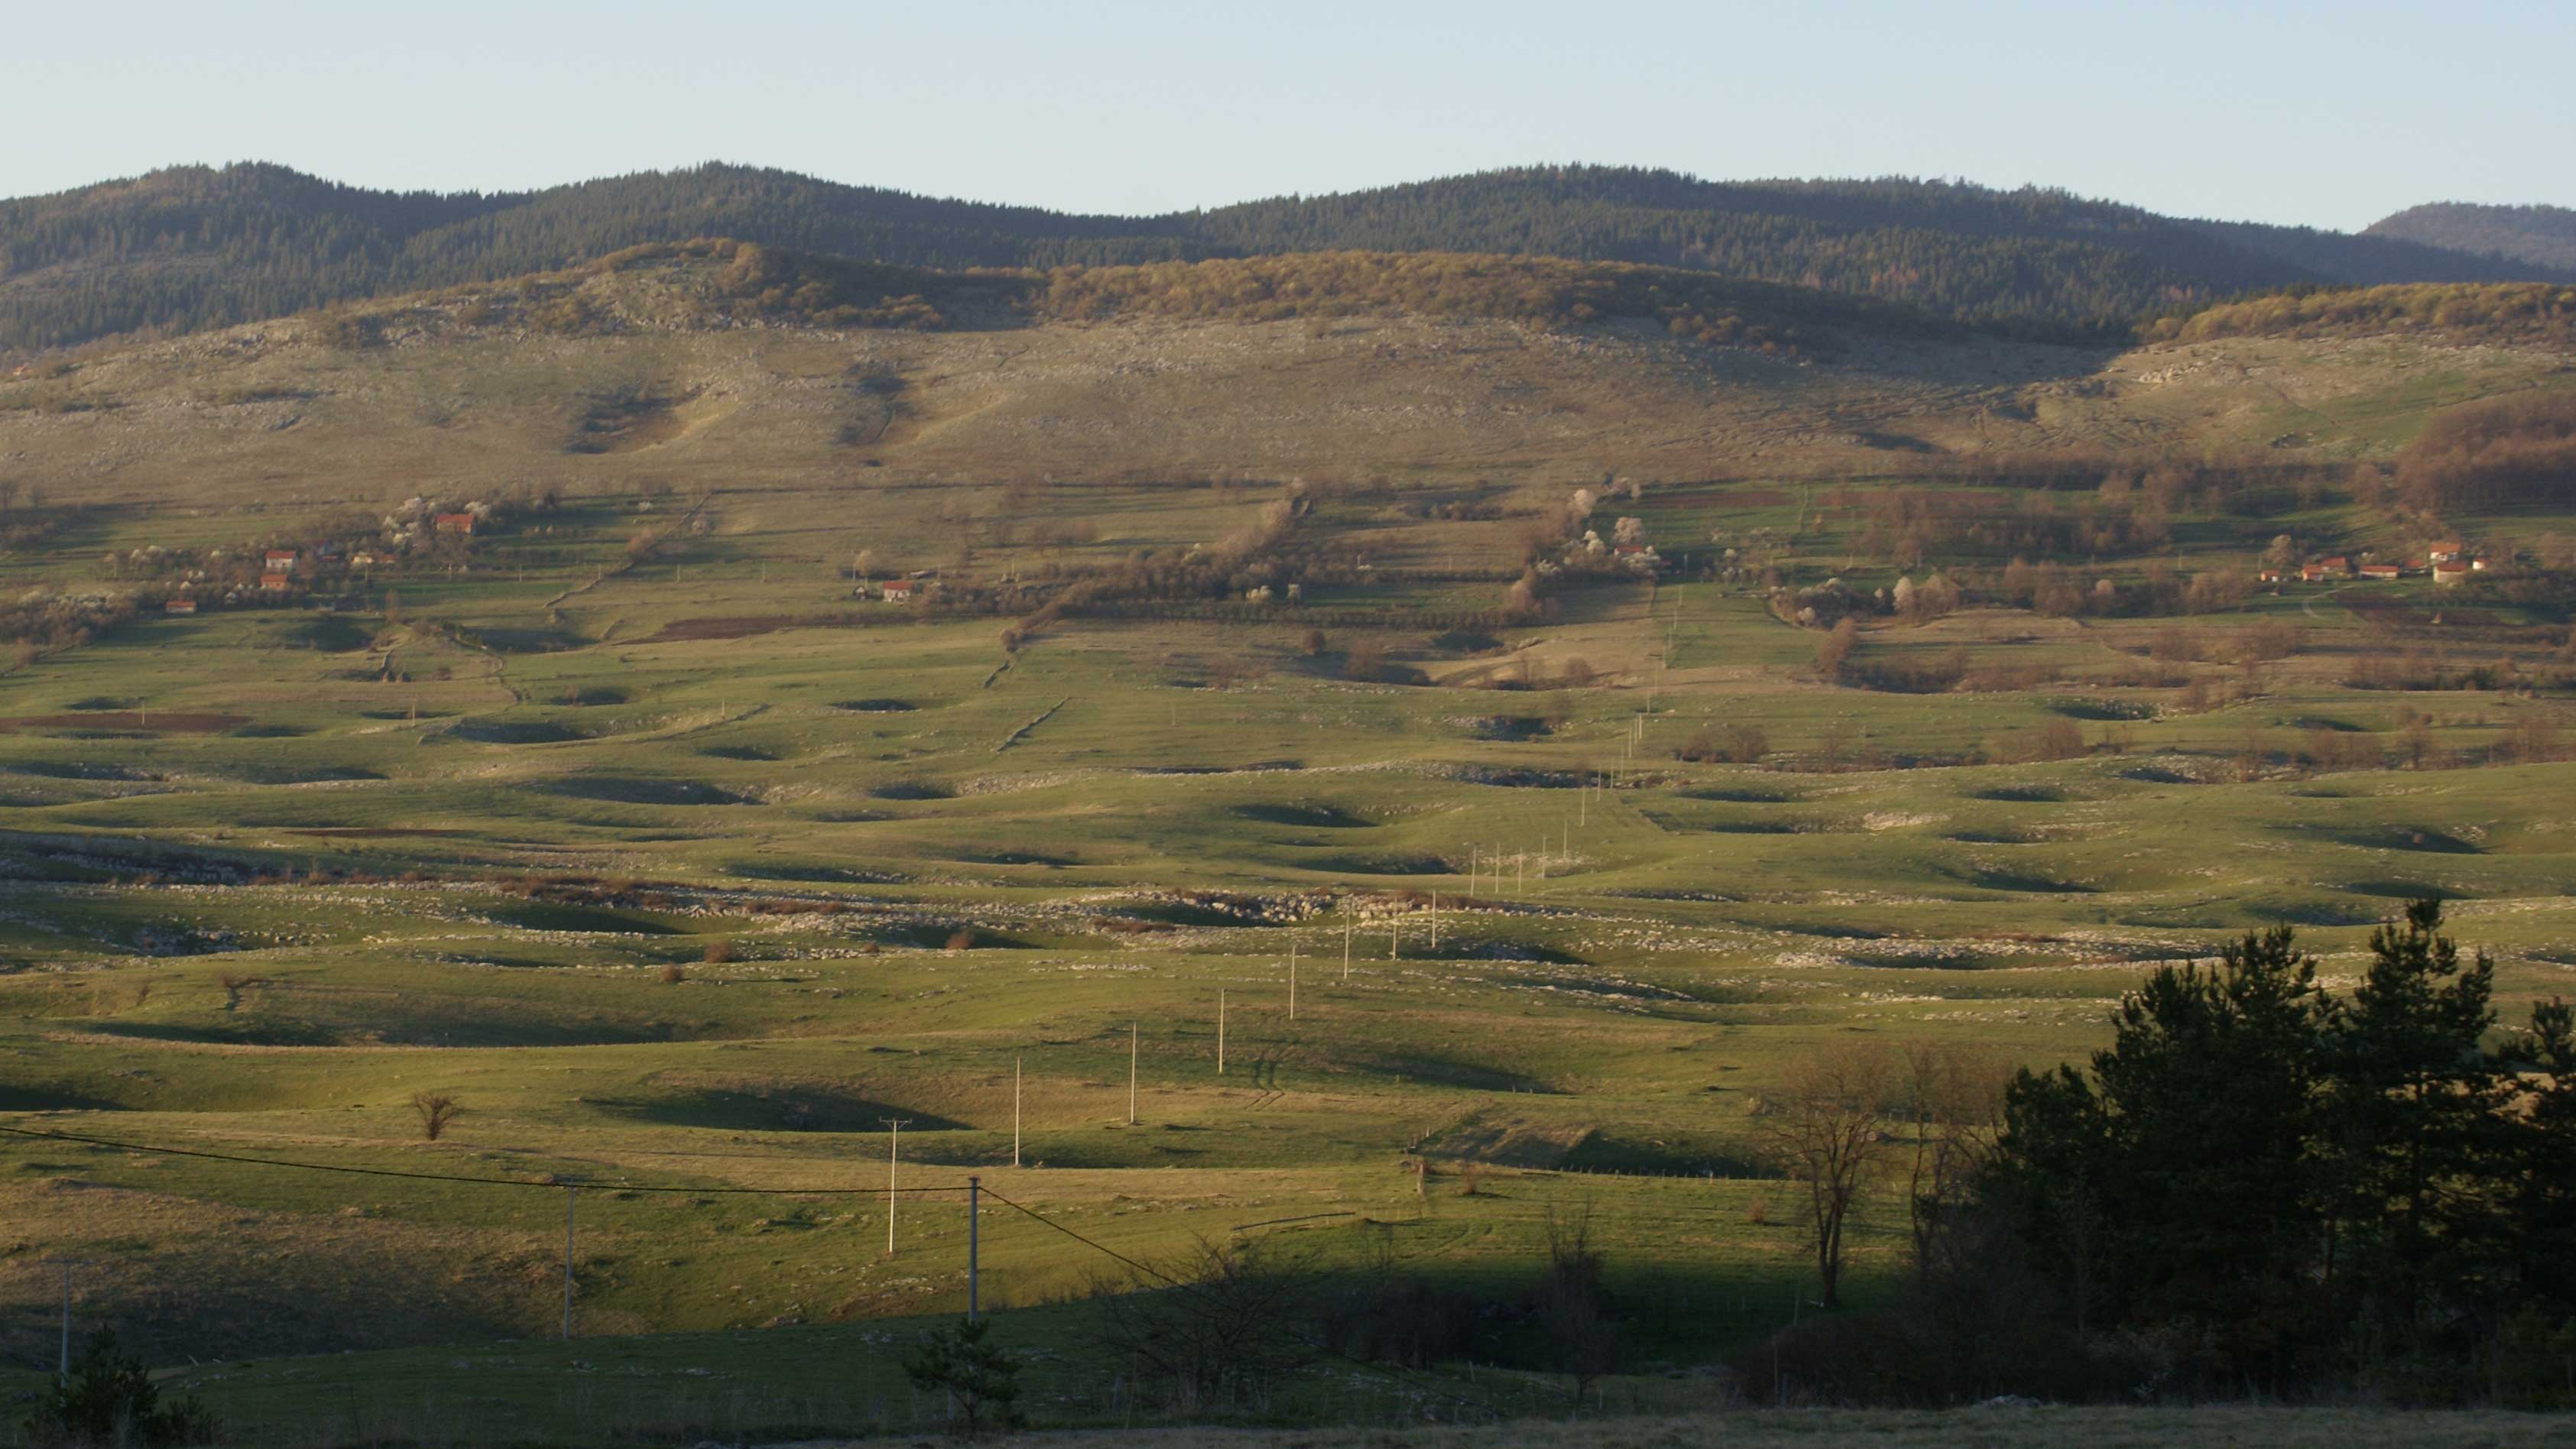
\includegraphics[width=1.15\textwidth]{slike/bpetrovac} \\
    Kapljuh, BiH \small{(vir: A.M.)}
  \end{center}
\end{frame}

\begin{comment}
\begin{frame}{Kraške vrtače}{Več predlaganih modelov nastanka}
  \begin{center}
    \hspace*{-0.075\textwidth}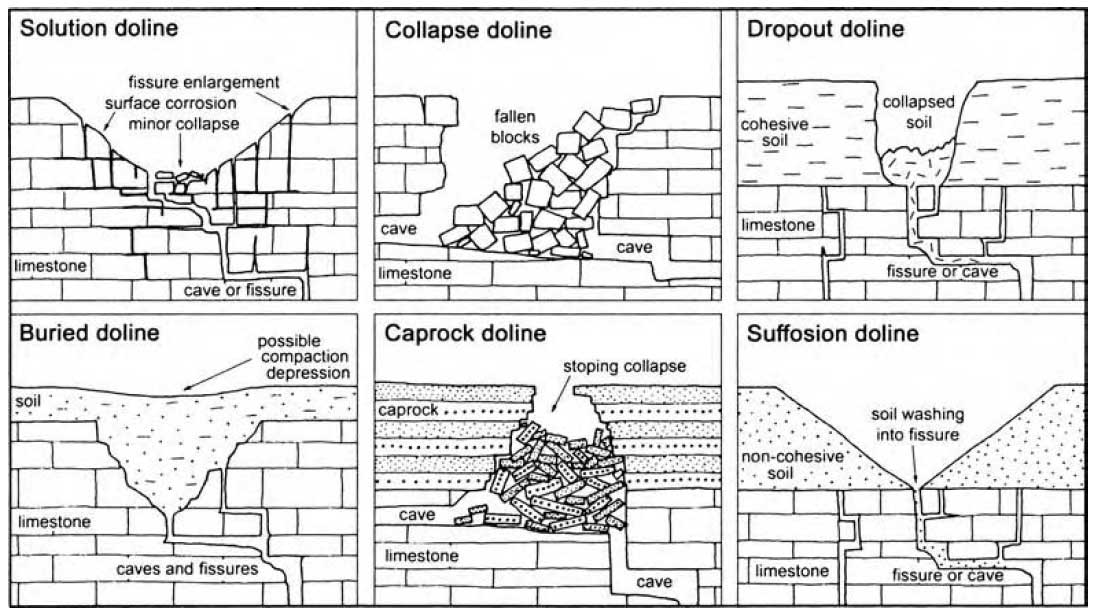
\includegraphics[width=1.10\textwidth]{slike/nastanek}
  \tiny{\\Vir: Ford, Williams, Karst Hydrogeology and Geomorphology}
  \end{center}
\end{frame}
\end{comment}

\begin{comment}
\begin{frame}{Kraške vrtače}{Več predlaganih modelov nastanka}
  \begin{center}
    \hspace*{-0.1\textwidth}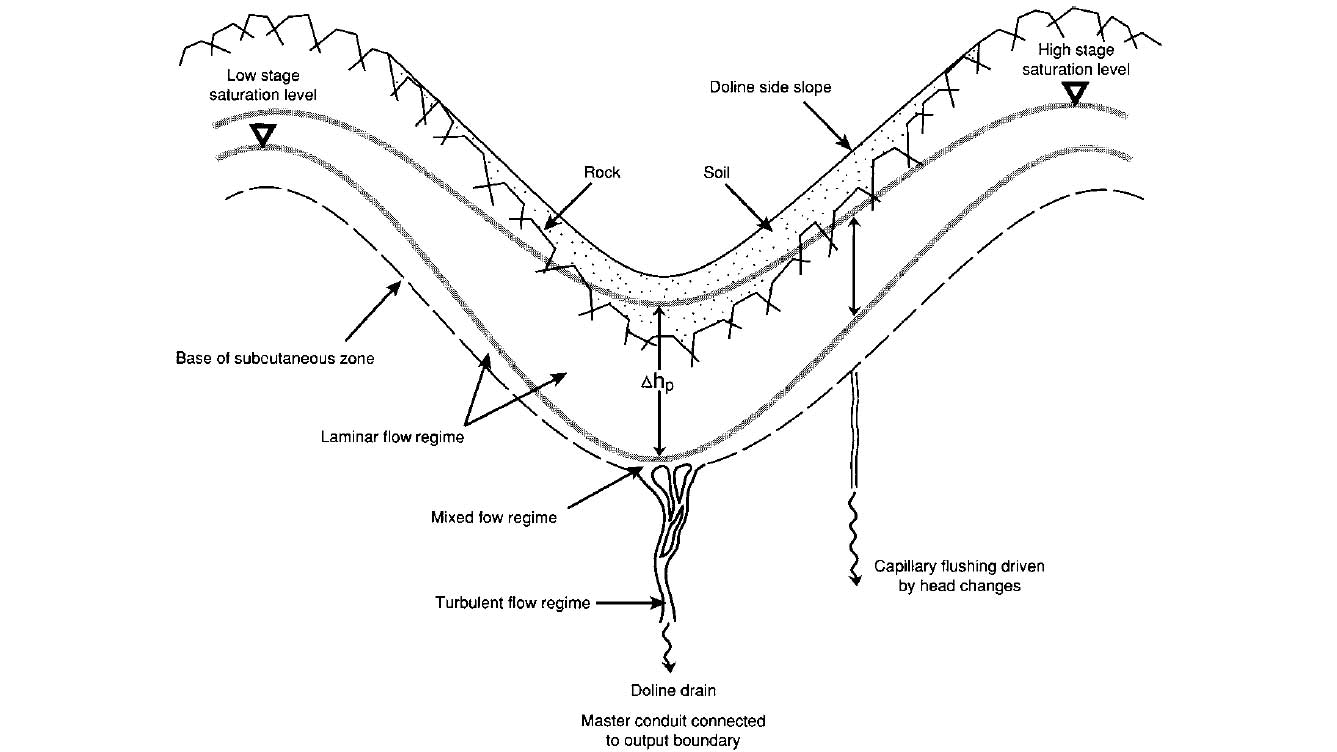
\includegraphics[width=1.2\textwidth]{slike/nastanek2}
  \end{center}
\end{frame}
\end{comment}

\begin{frame}{Kraške vrtače}{Ni podrobnejših študij procesov, ki jih oblikujejo}

\begin{columns}
  \begin{column}{0.6\textwidth}
    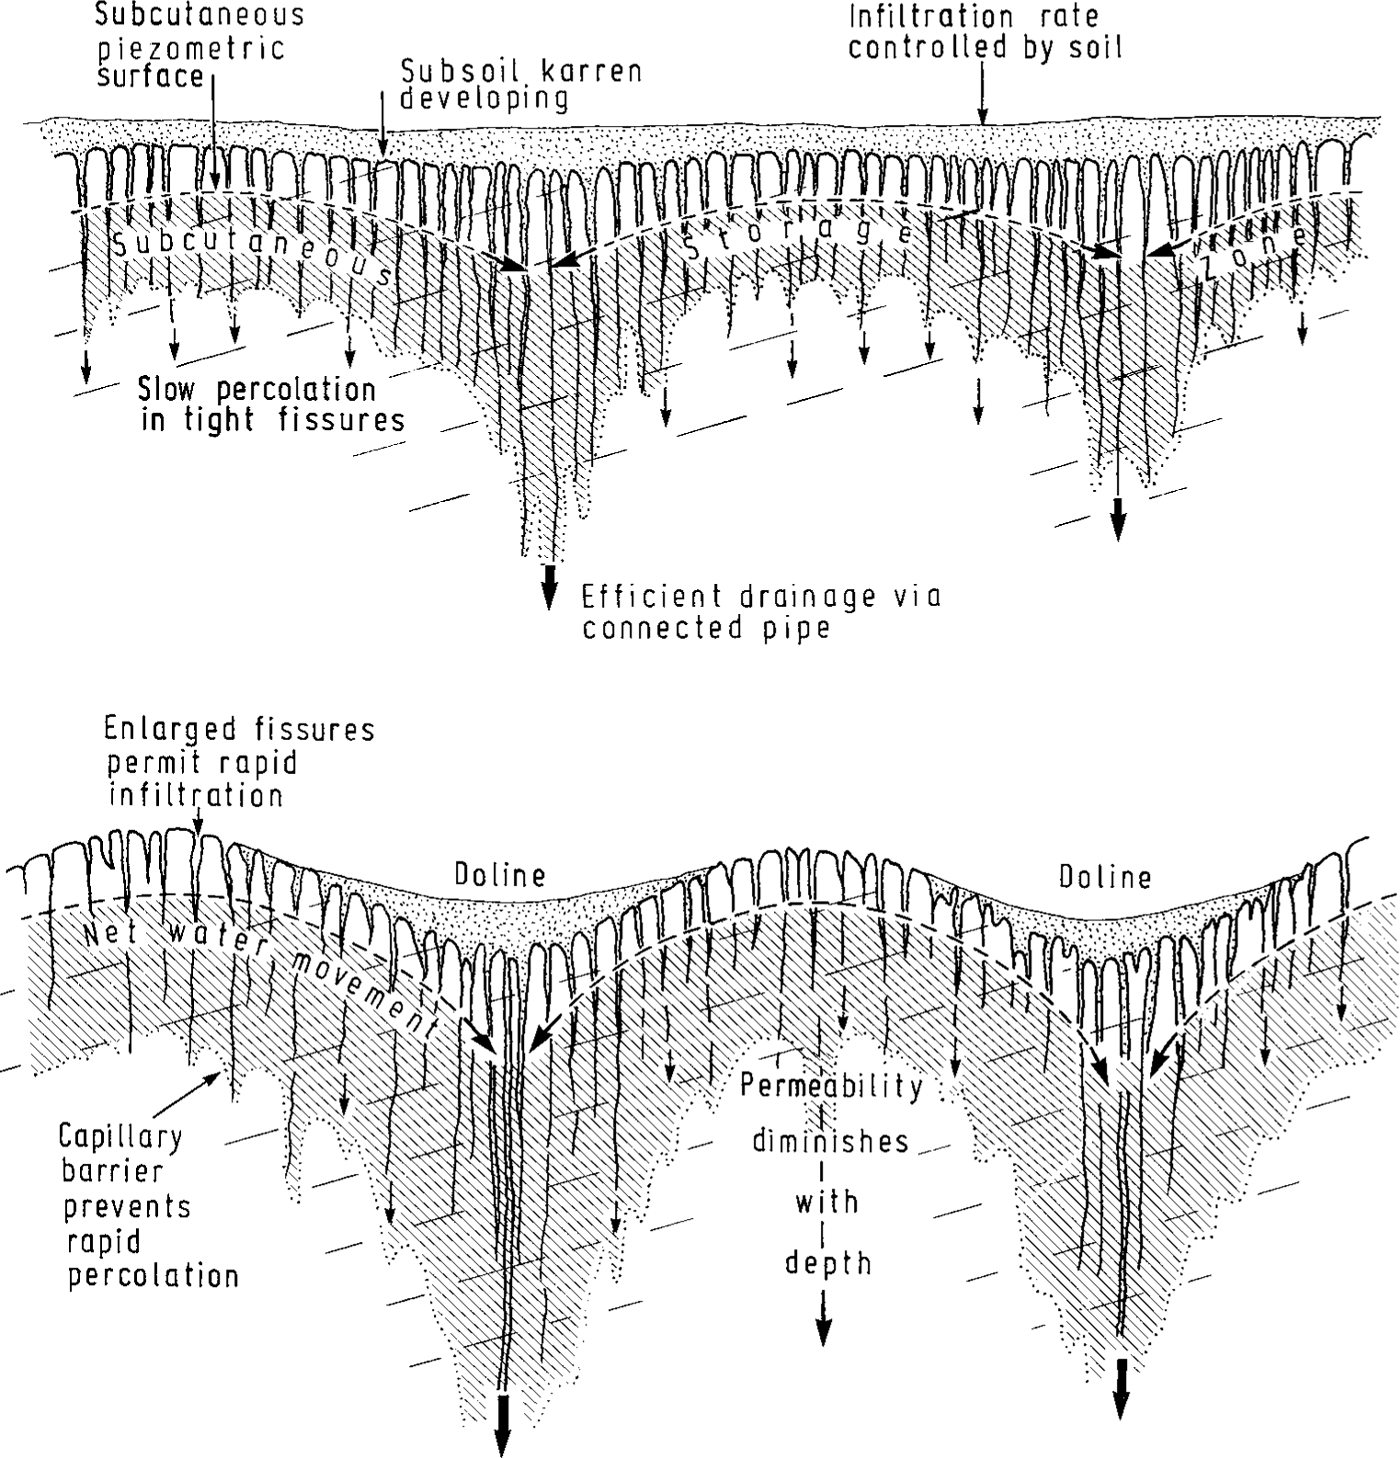
\includegraphics[width=\textwidth]{slike/vrtaca-ford-williams}
    \tiny{\\Vir: Ford, Williams, Karst Hydrogeology and Geomorphology}
  \end{column}

  \begin{column}{0.5\textwidth}
    \includegraphics[width=\textwidth]{slike/verd}
    \tiny{\\Vir: A.M}
  \end{column}
\end{columns}
\end{frame}


\begin{frame}{Kraške vrtače}{LiDARski posnetek območja Menišije, ločljivost $1m^2$ \\ Površina $\approx 7 km$ x $14 km$ \\ Število vrtač $\approx 8700$ \\ Starost površja = $0,5 - 3,5$ milijonov let}
\begin{center}
  \hspace*{-1cm}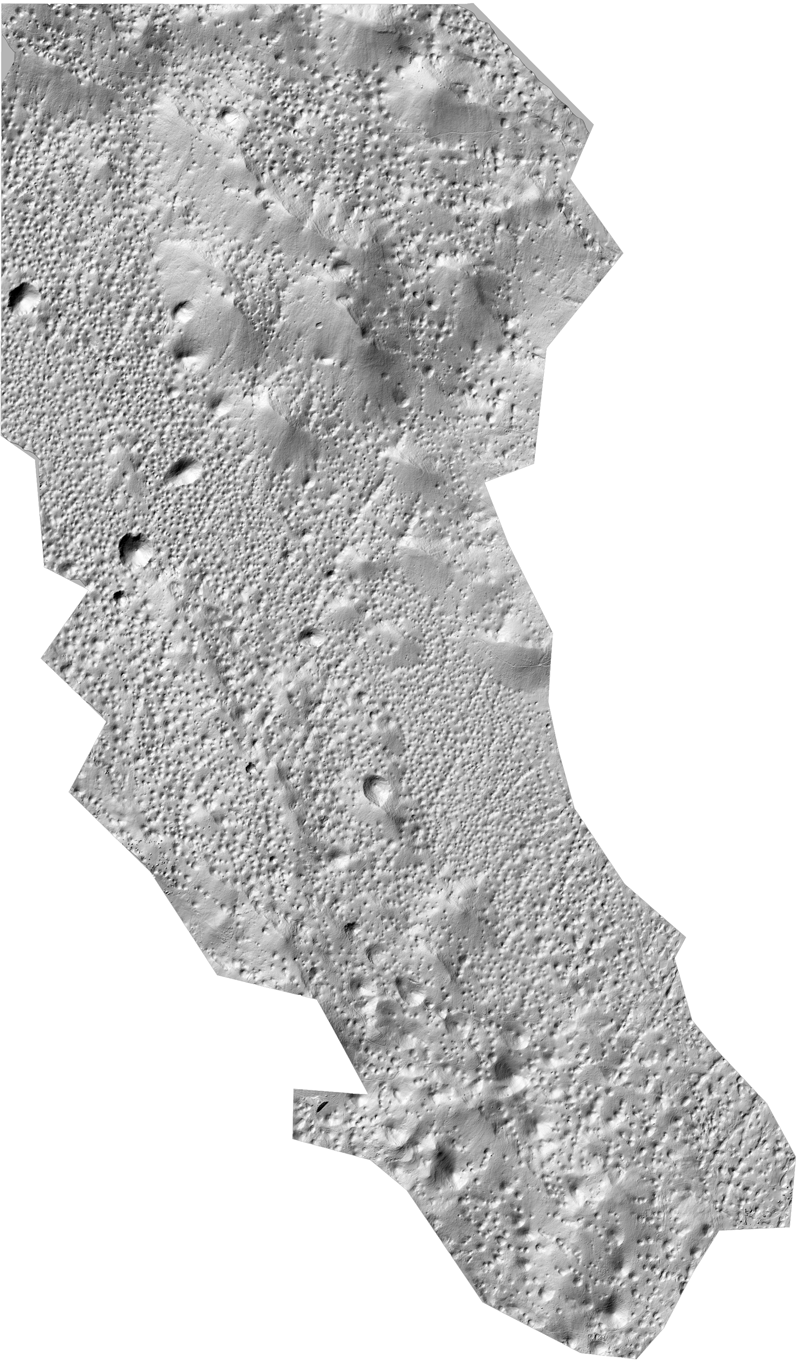
\includegraphics[width=0.62\textwidth,angle=90]{slike/menisija-relief}
  \tiny{\\Vir podatkov: Gozdarski inštitut Slovenije}
\end{center}
\end{frame}

\subsection{Indeks konkavnosti}

\begin{frame}{Indeks konkavnosti}{Definicija $I_k$}

\begin{columns}
  \begin{column}{0.5\textwidth}
    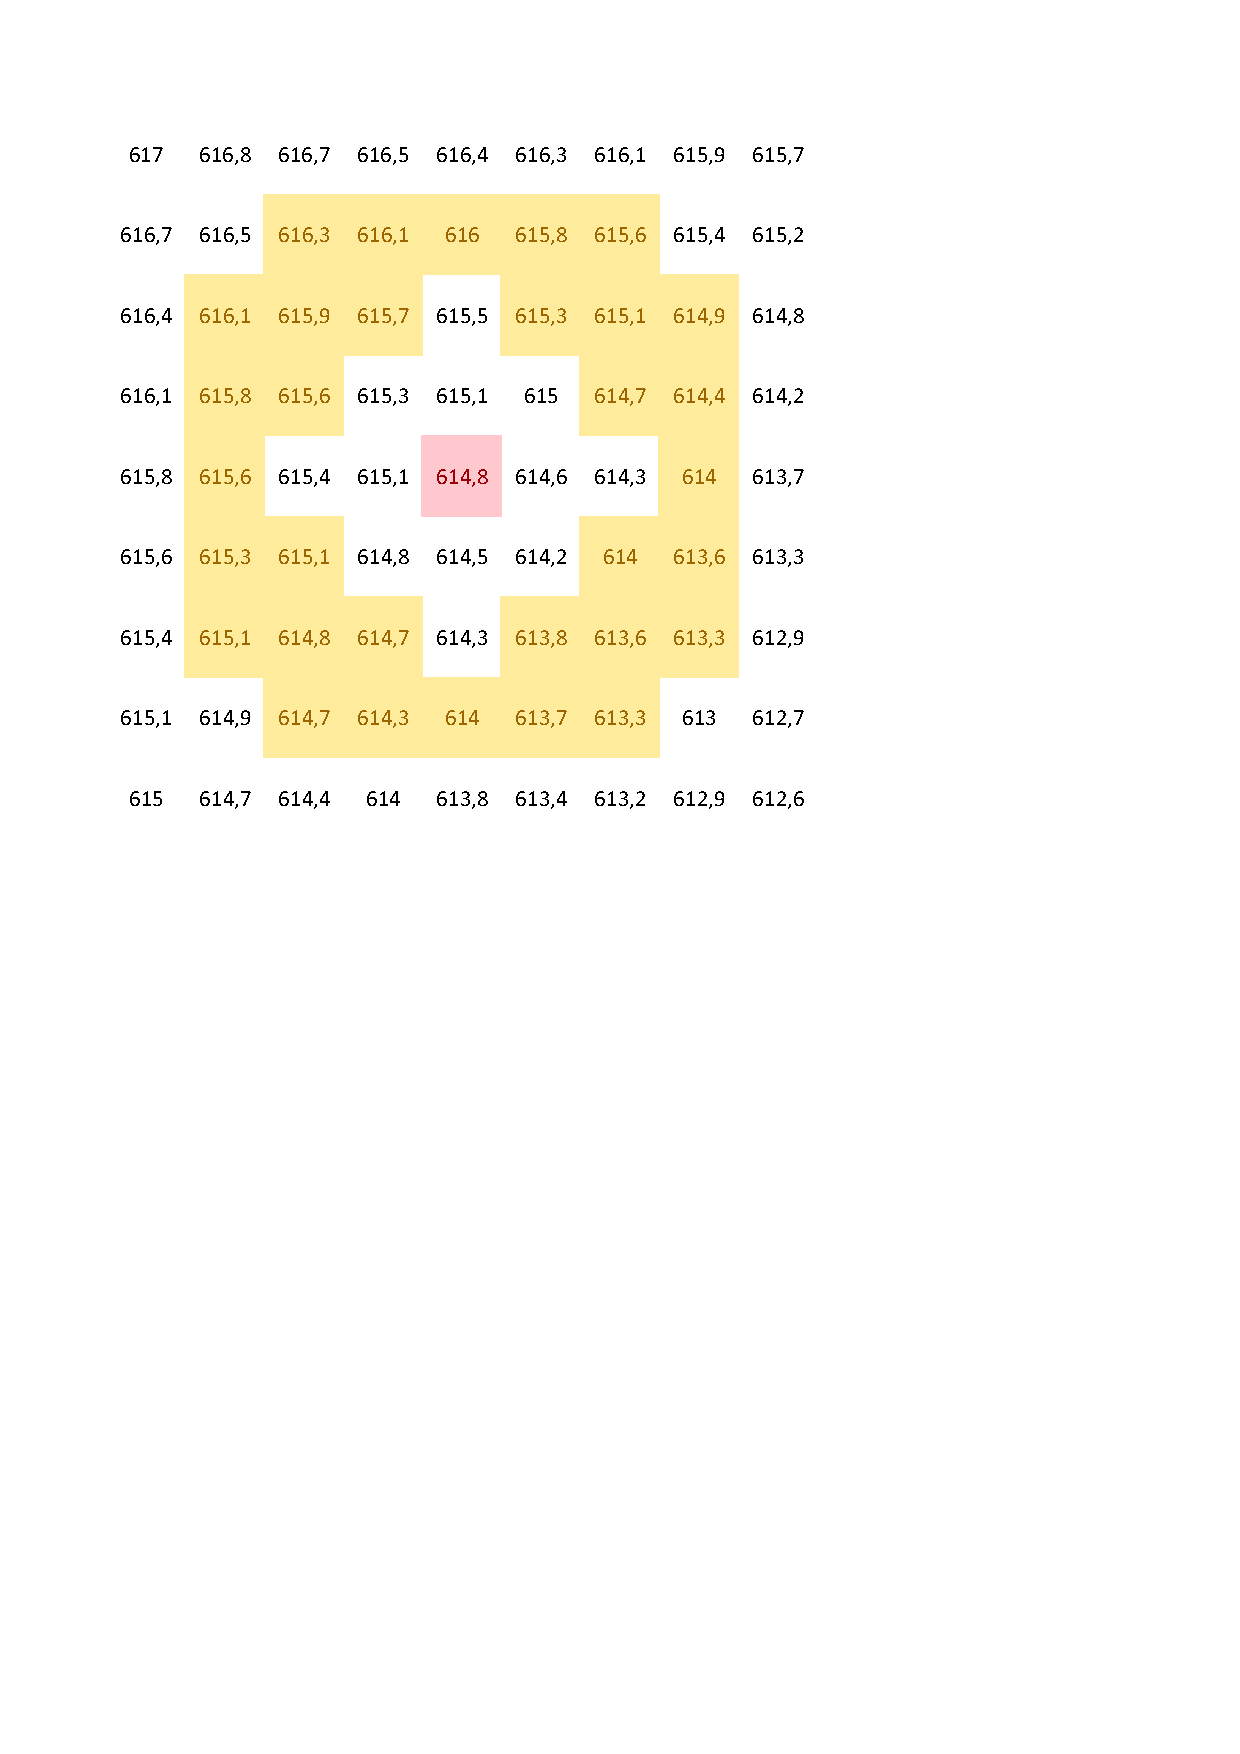
\includegraphics[width=\textwidth]{slike/concavity-ring-visualisation-2}
  \end{column}
  \begin{column}{0.6\textwidth}
  \footnotesize
  \begin{equation}  I_k(r_0,r_1,r_2) = h(r_0)- \frac{1}{N}\sum\limits_{r_1<r<r_2} h(r) \label{ik} \end{equation}
  \end{column}
\end{columns}

\end{frame}

\begin{frame}{Indeks konkavnosti}{Indeks konkavnosti za različne dimenzije kolobarja ($r_1$, $r_2$)}
    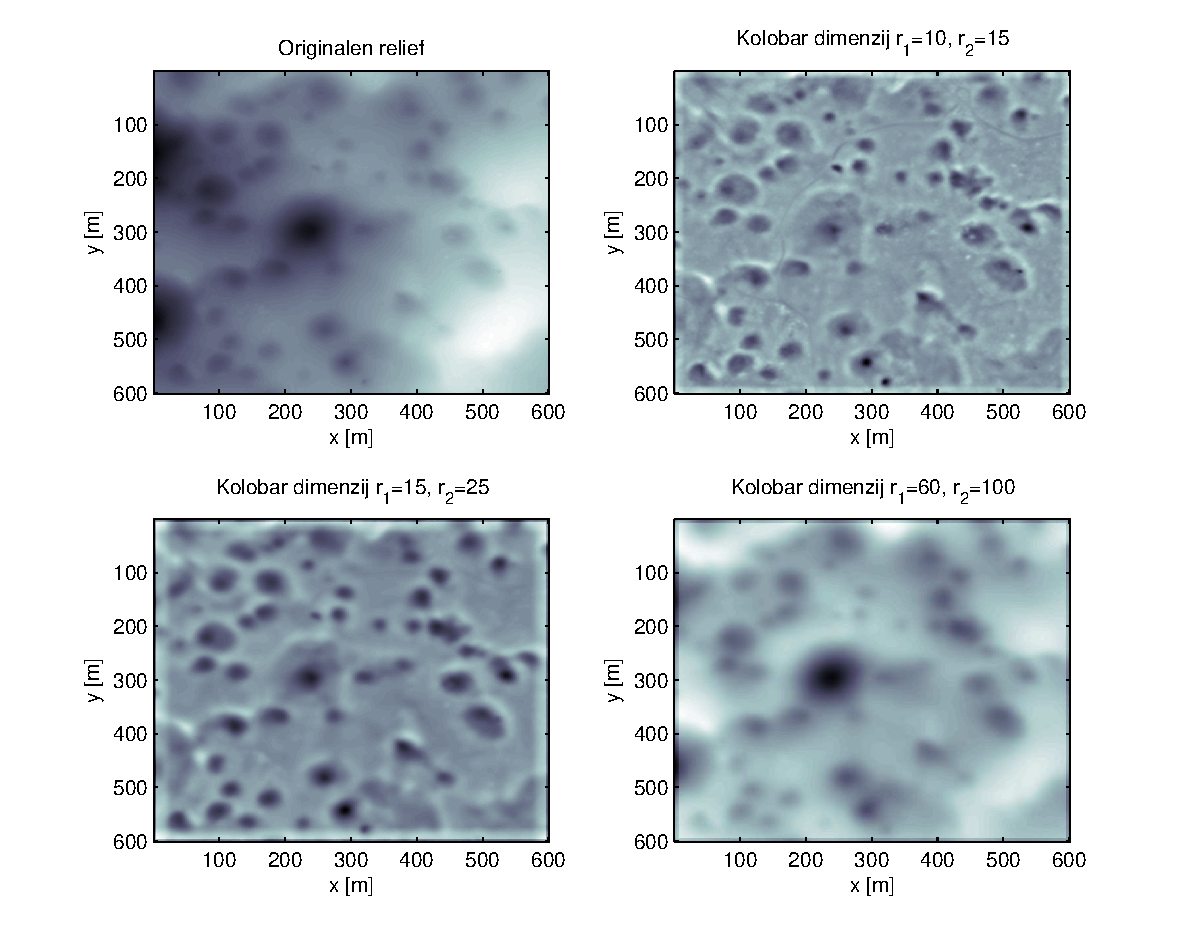
\includegraphics[width=\textwidth]{slike/concavity-samples}
\end{frame}

\begin{frame}{Indeks konkavnosti}{Za vrtače odberemo površje kjer $I_k > \frac{\sigma_{I_k}}{2}$}
    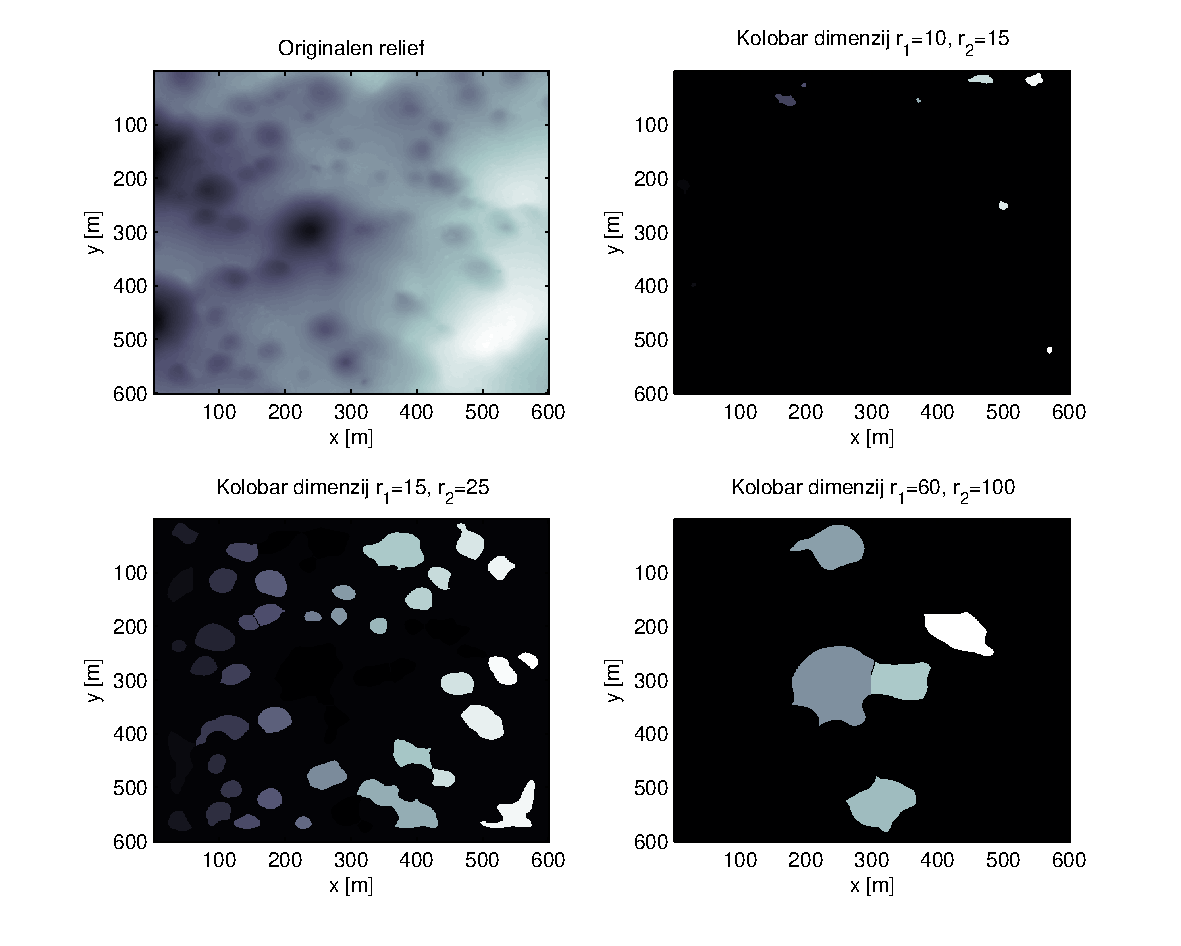
\includegraphics[width=\textwidth]{slike/concavity-segmentation-samples}
\end{frame}

\begin{frame}{Indeks konkavnosti}{Rezultat odbiranja konkavnosti}
\begin{columns}
  \begin{column}{0.55\textwidth}
    \hspace*{-0.02\textwidth}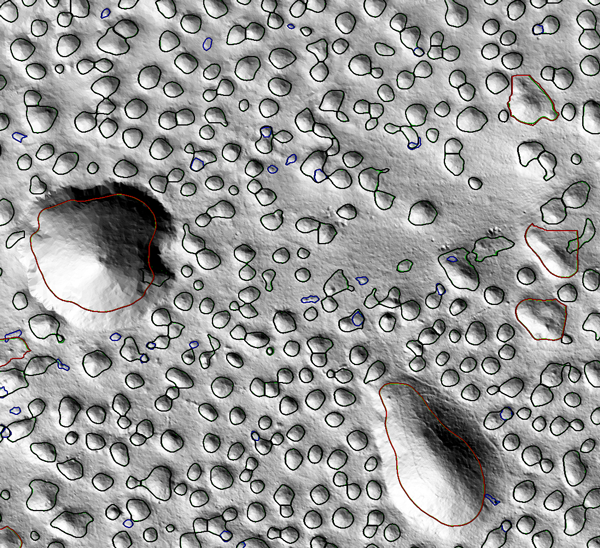
\includegraphics[width=\textwidth]{slike/menisija-vrtace}
  \end{column}

  \begin{column}{0.5\textwidth}
    \hspace*{-0.15\textwidth}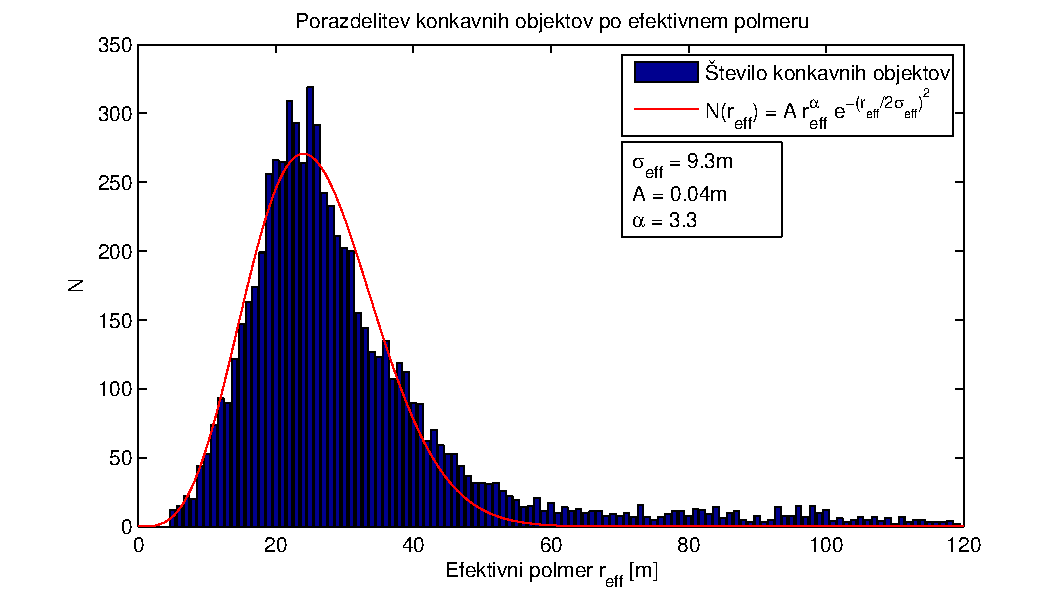
\includegraphics[width=1.3\textwidth]{slike/menisija-polmeri-hist-maxwell}
    \footnotesize
    \begin{equation} A = \sum piksli \end{equation}
    \begin{equation}r_{eff} = \sqrt{\frac{A}{\pi}} \end{equation}
  \end{column}
\end{columns}
\end{frame}

\subsection{Oblika vrtače}

\begin{frame}{Oblika vrtače}{Izračunamo povprečno vrtačo (levo) in standardno deviacijo najdenih vrtač (desno)\\Uporabimo Gaussovo funkcijo za njihov opis}
  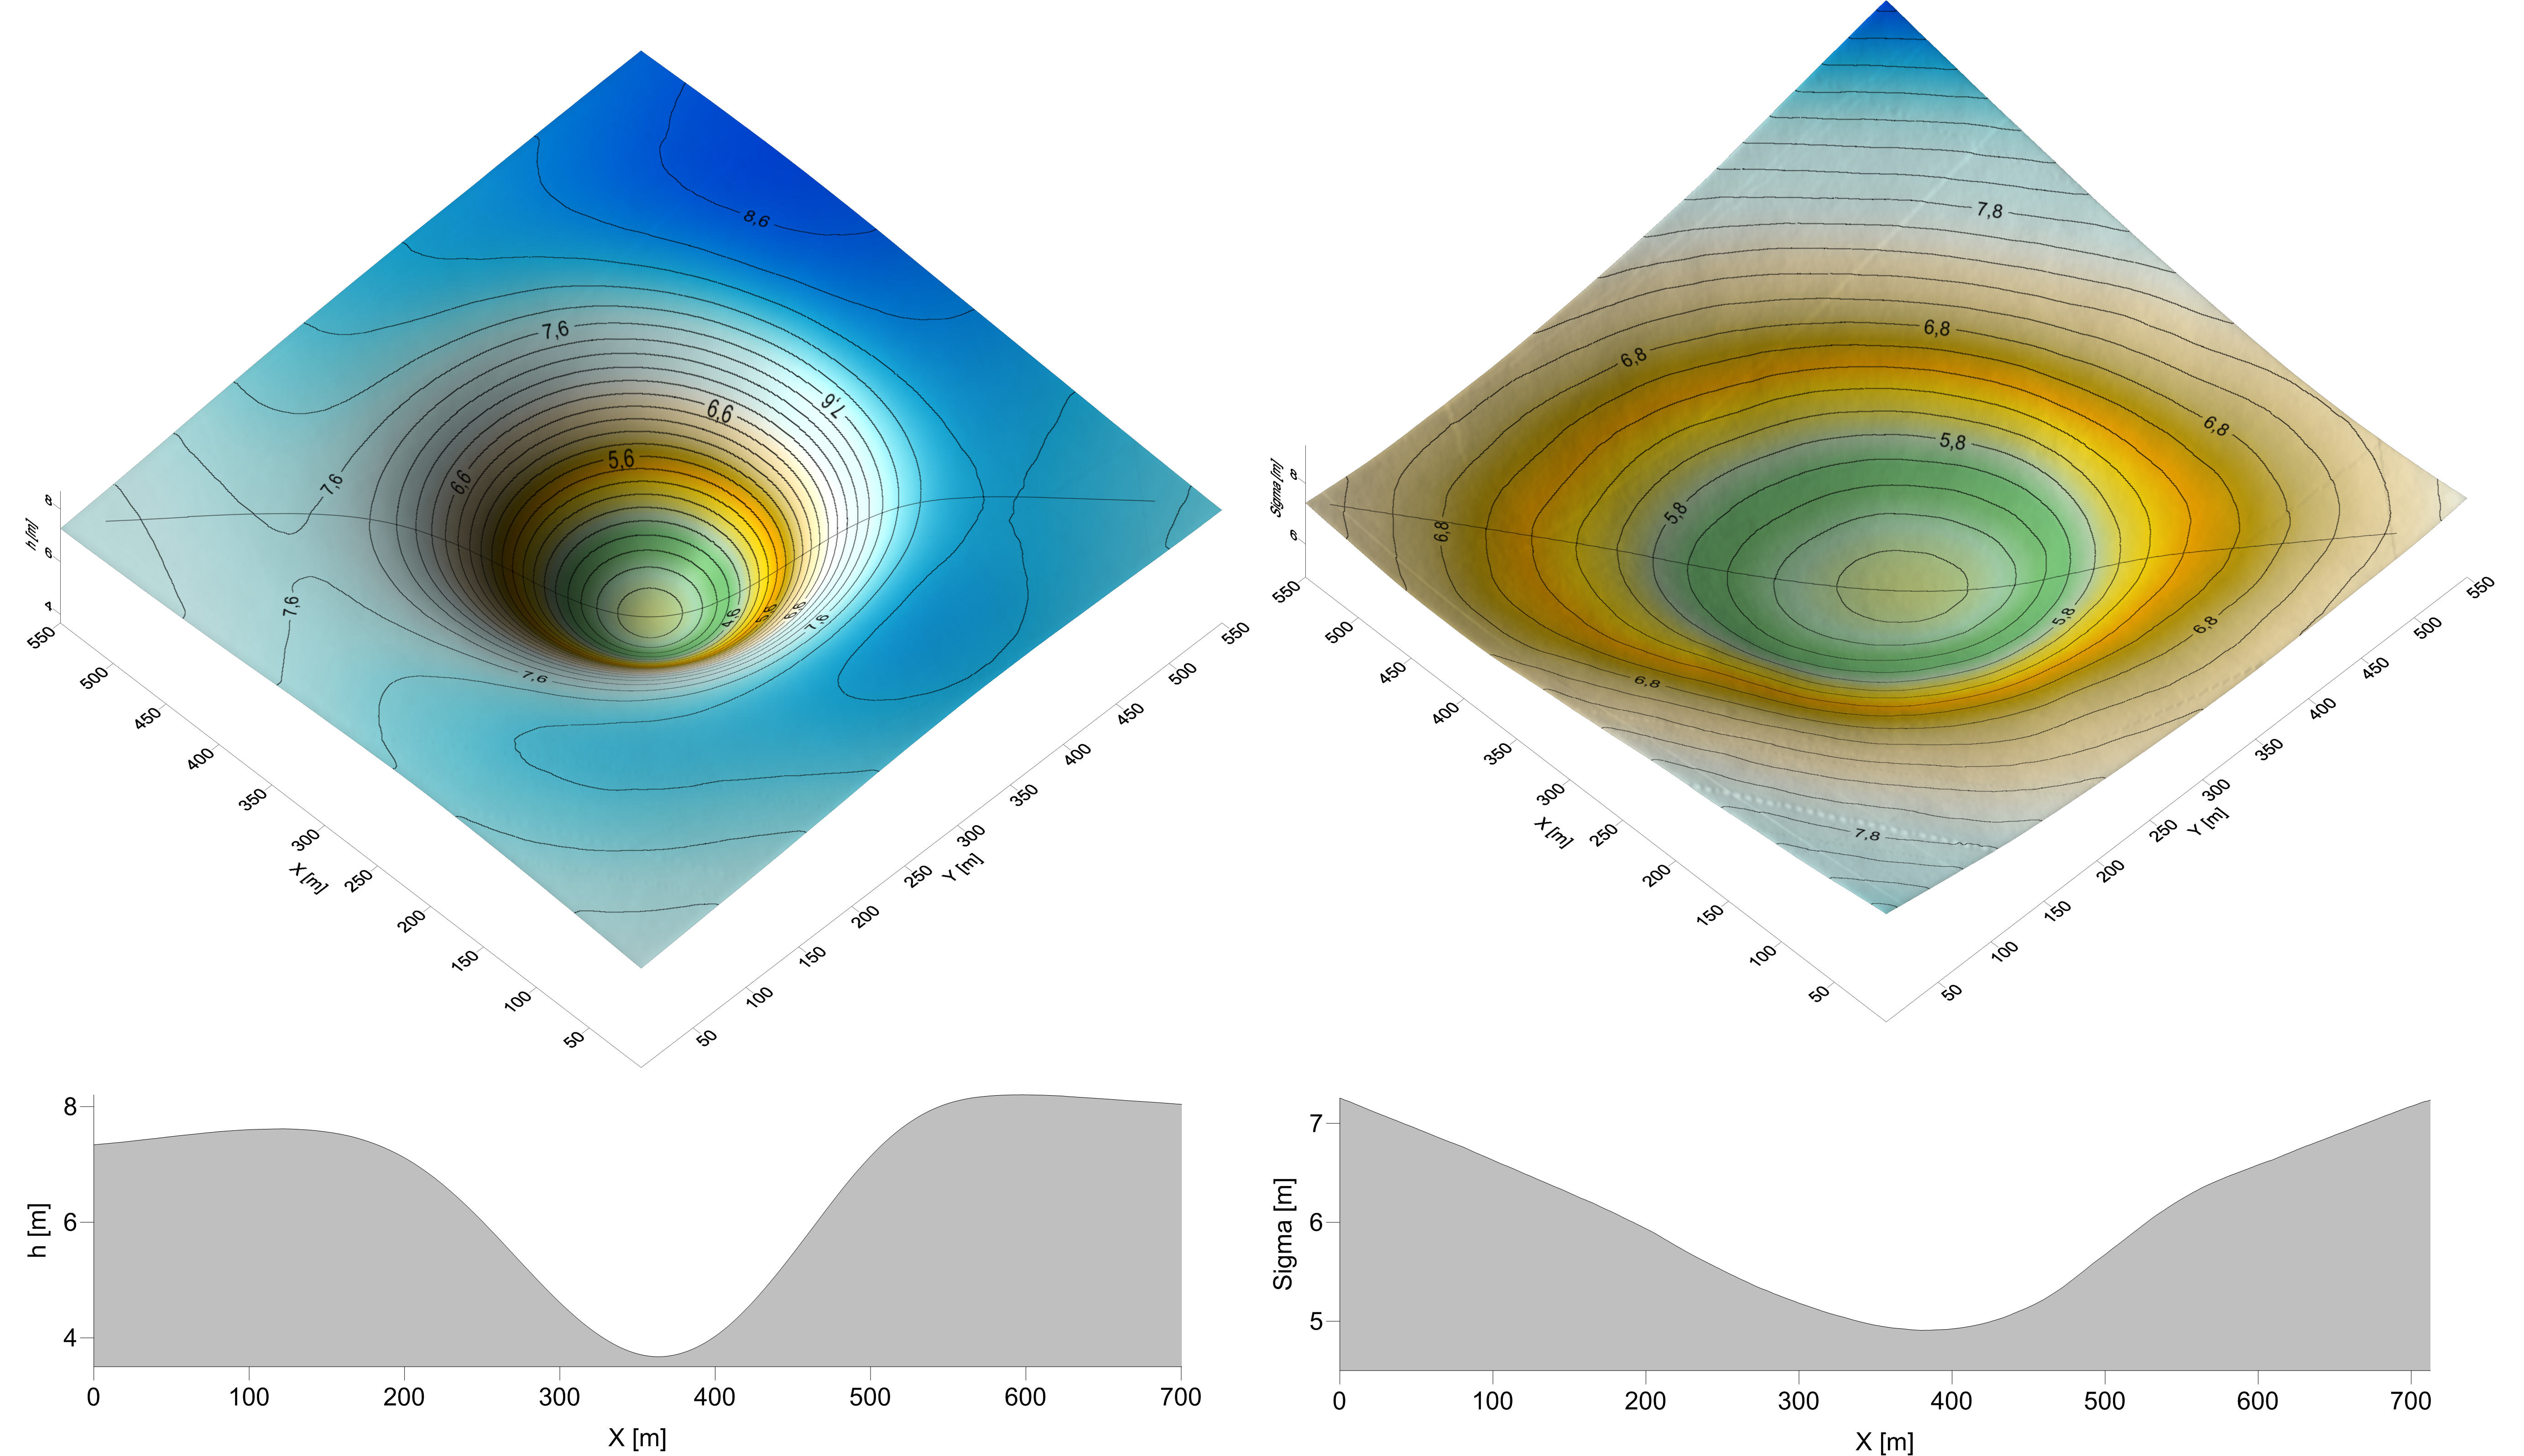
\includegraphics[width=\textwidth]{slike/menisija-vrtaca-sigma}
  \begin{equation} h(r) = A \cdot e^{-\frac{(r-r_0)^2}{\sigma^2}} + C \end{equation}
\end{frame}

\begin{frame}{Oblika vrtače}{Odberemo vrtače za katere $23,5m < r_{eff} < 24,5m$ \\ izračunamo njihove profile $\bar h_i(r)$ \\ izračunamo povprečen profil $\bar H(r)$ in odstopanje prilegane Gausovke $f(r)$}
\begin{columns}
  \begin{column}{0.7\textwidth}
    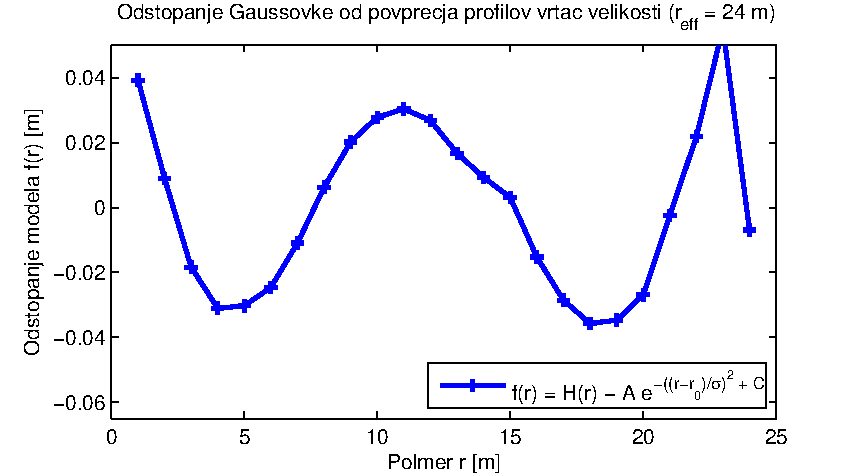
\includegraphics[width=1.05\textwidth]{slike/menisija-profil-21-fit}
  \end{column}
  \begin{column}{0.45\textwidth}
    \footnotesize
    \begin{equation} \bar h_i(r) = \frac{1}{2 \pi} \int_0^{2\pi} h_i(r,\phi) \mathrm{d}\phi \end{equation}
    \begin{equation} \bar H(r) = \frac{1}{N} \sum_{i} \bar h_i(r) \end{equation}
    \begin{equation} f(r) = \bar{H}(r) - A \cdot e^{-\frac{(r-r_0)^2}{\sigma^2}} + C \end{equation}
  \end{column}
\end{columns}
\end{frame}

\begin{frame}{Oblika vrtače}{Vsem vrtačam prilegamo Gaussovko in prikažemo histograma za $A$ in $\sigma$}
    \hspace*{-0.1\textwidth}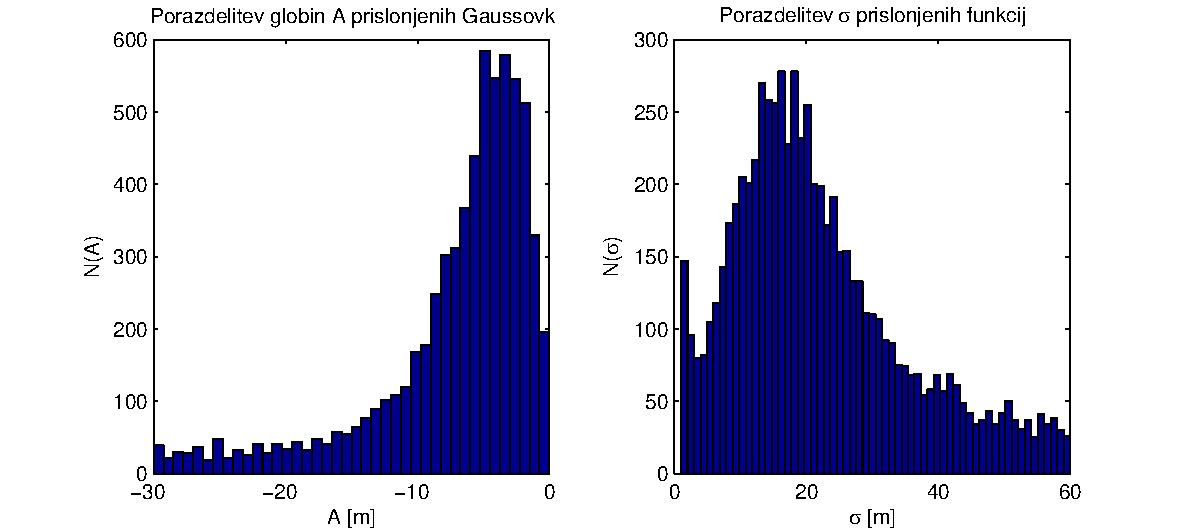
\includegraphics[width=1.2\textwidth]{slike/menisija-visine-in-sigme-hist}
\end{frame}

\begin{frame}{Oblika vrtače}{Vsem vrtačam prilegamo Gaussovko in prikažemo odvisnosti za $\sigma(r_{eff})$, $|A(r_{eff})|$ in $|A(\sigma)|$}
    \hspace*{-0.1\textwidth}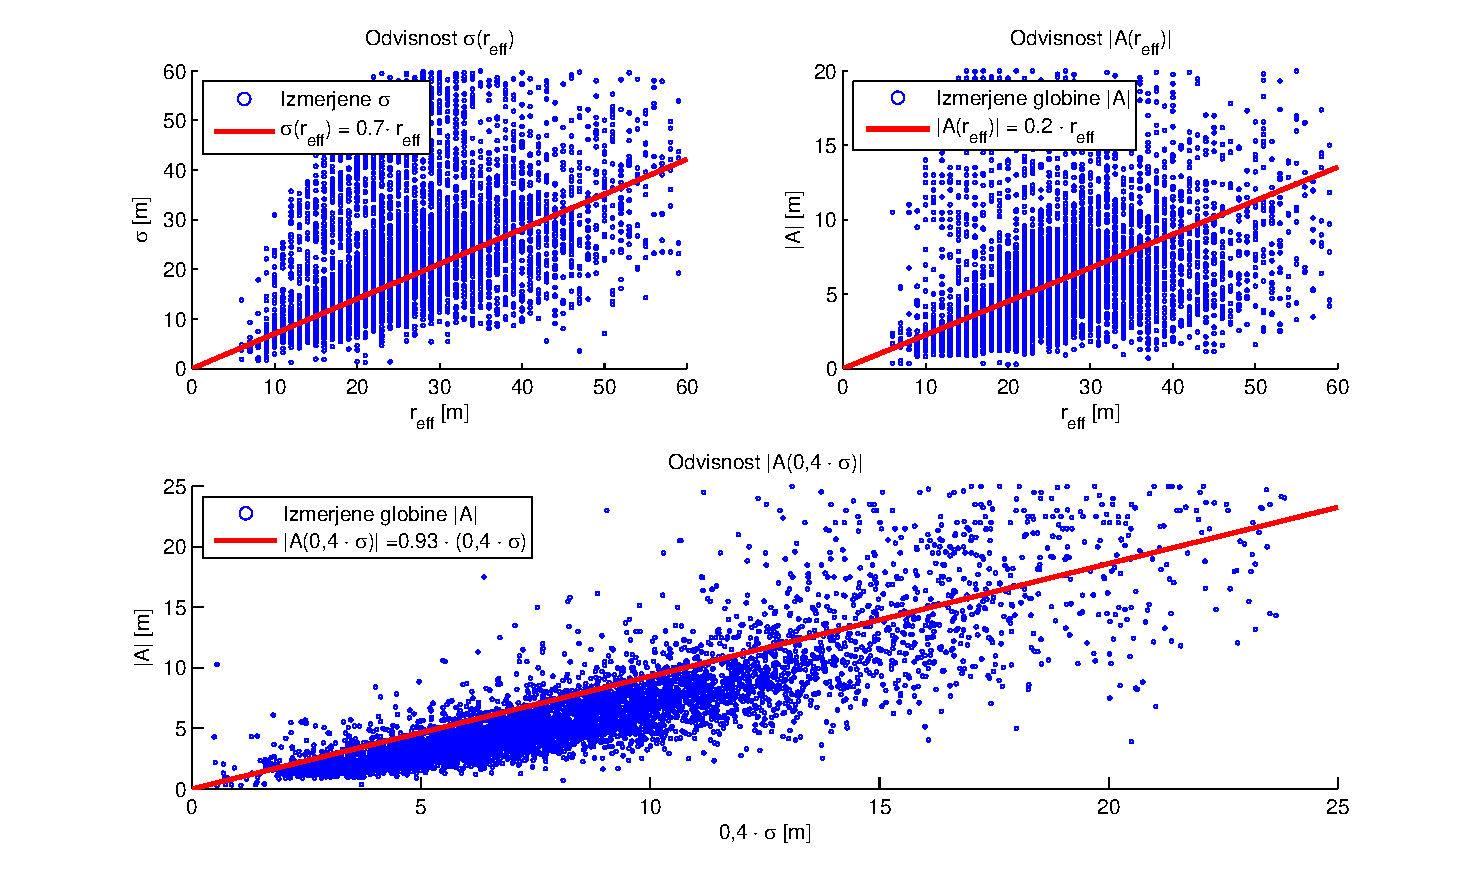
\includegraphics[width=1.2\textwidth]{slike/menisija-A-sigma-reff}
\end{frame}

\section{Rast površin}

\subsection{Opis rasti površin}

\begin{frame}{Opis rasti površin}{Hrapavost površine $w(L,t)$, priraščanje $\langle h(t) \rangle$}
\begin{columns}
  \begin{column}{0.45\textwidth}
     \hspace*{-0.05\textwidth}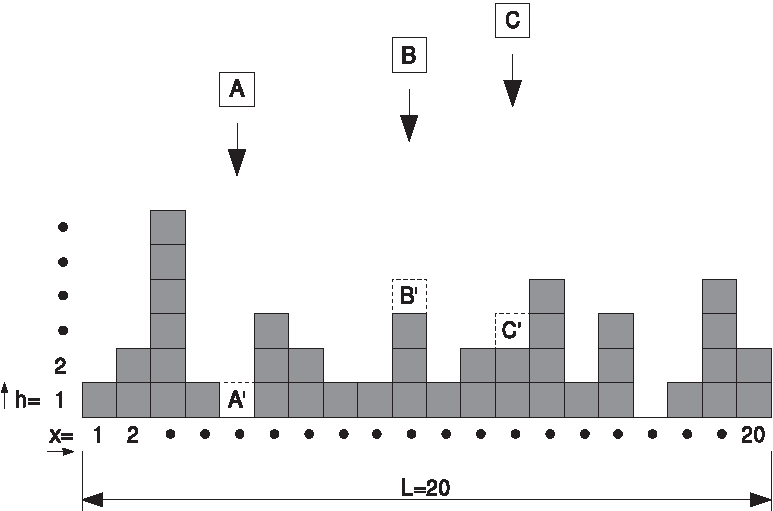
\includegraphics[width=1.1\textwidth]{slike/bdep2.pdf}
     \newline
     \newline
     \tiny{Vir: A. Schwettmann, Ballistic deposition: Global scaling and local time series}
     \newline \newline
     \tiny{(V primeru vrtač material odvzemamo. Problem je matematično enak.)}
  \end{column}

  \begin{column}{0.55\textwidth}
    \footnotesize
    \begin{equation} p(x) = \frac{1}{L} \end{equation}
    \newline
    \begin{equation} \langle h(t) \rangle = \frac{1}{L} \sum_{i=1}^L h(x,t) \end{equation}
    \newline
    \begin{equation} w(L,t) = \sqrt{\frac{1}{L} \sum_{i=1}^L (h(x,t)-\bar{h}(t))^2} \end{equation}
    \newline
    \begin{equation} \langle h(t) \rangle \sim t \end{equation}
  \end{column}
\end{columns}
\end{frame}


\begin{frame}{Opis rasti površin}{Pričakovana hrapavost površine $\langle w(L,t) \rangle$, eksponent hrapavosti $\alpha$}
\begin{center}
  \footnotesize
  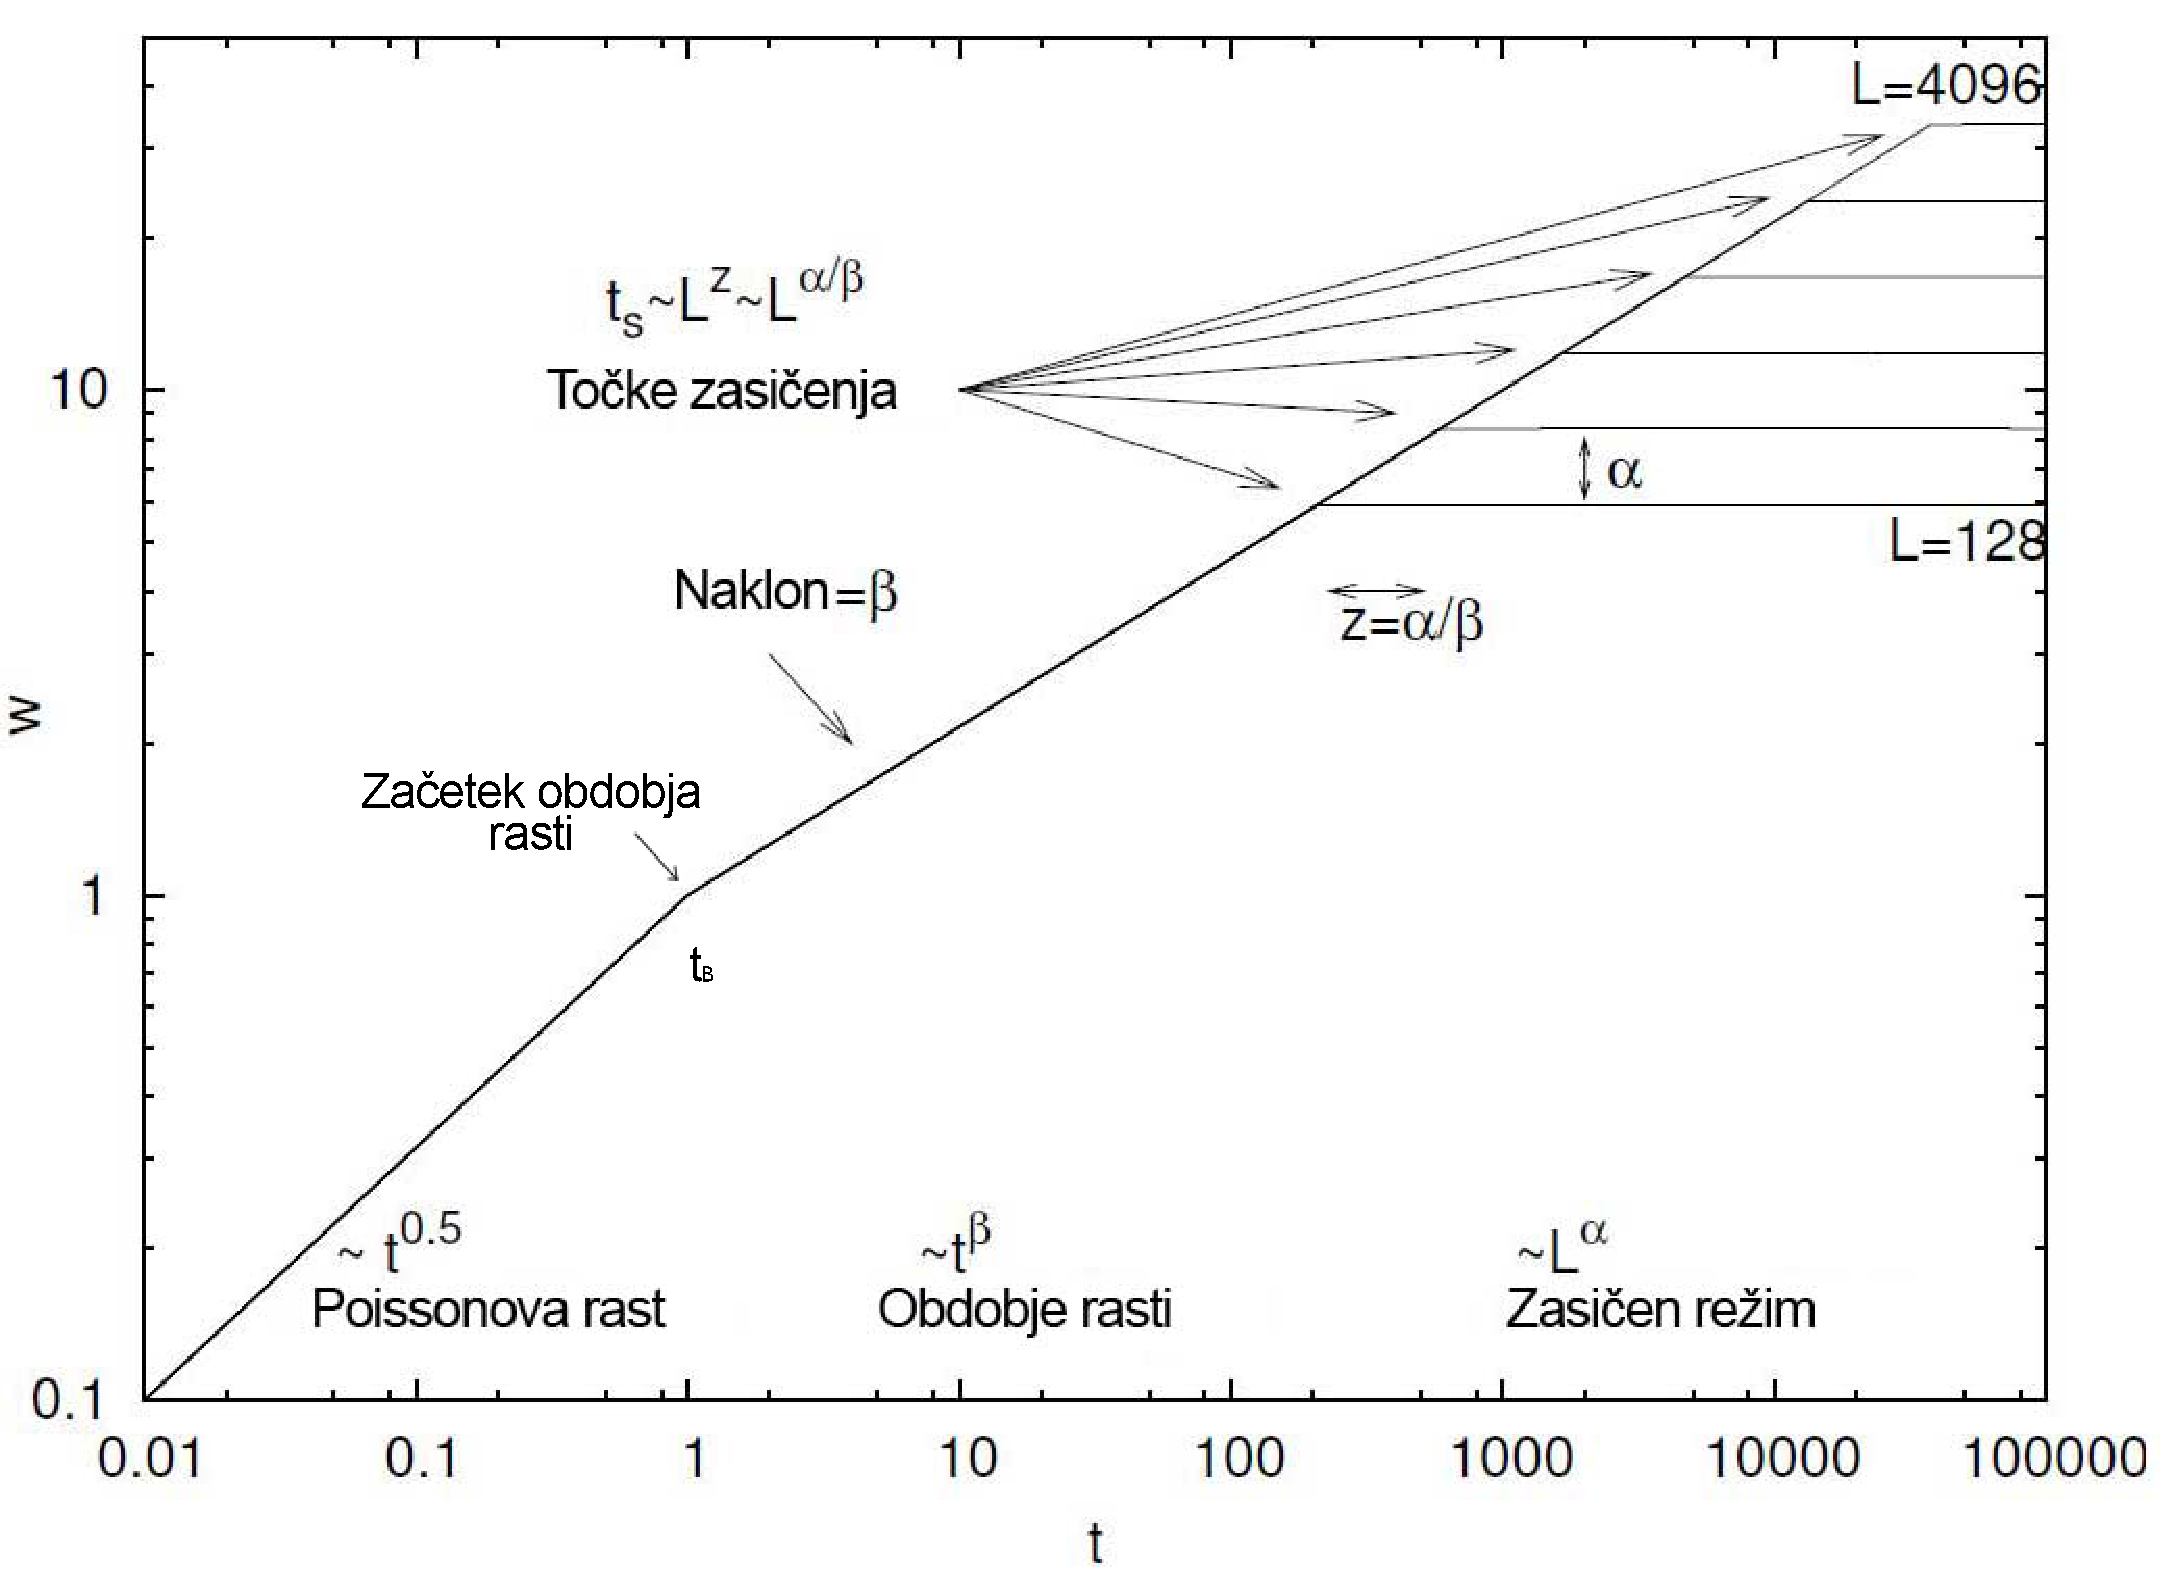
\includegraphics[width=0.8\textwidth]{slike/bdep3}
  \\ \tiny{Vir: A. Schwettmann, Ballistic deposition: Global scaling and local time series}
  \newline

\begin{columns}
  \begin{column}{0.6\textwidth}
    \begin{equation} w(L,t) = \left\langle \sqrt{\frac{1}{L} \sum_{i=1}^L (h(x,t)-\bar{h}(t))^2} \right\rangle \end{equation}
  \end{column}
  \begin{column}{0.4\textwidth}
    \begin{equation} \begin{array}{lr} w_{sat}(L) \sim L^\alpha & \ t \gg t_s \end{array} \end{equation}
  \end{column}
\end{columns}
\end{center}
\end{frame}

\begin{frame}{Opis rasti površin}{Izmerjen eksponent hrapavosti Menišije}
\begin{center}
  \footnotesize
  \hspace*{-0.04\textwidth}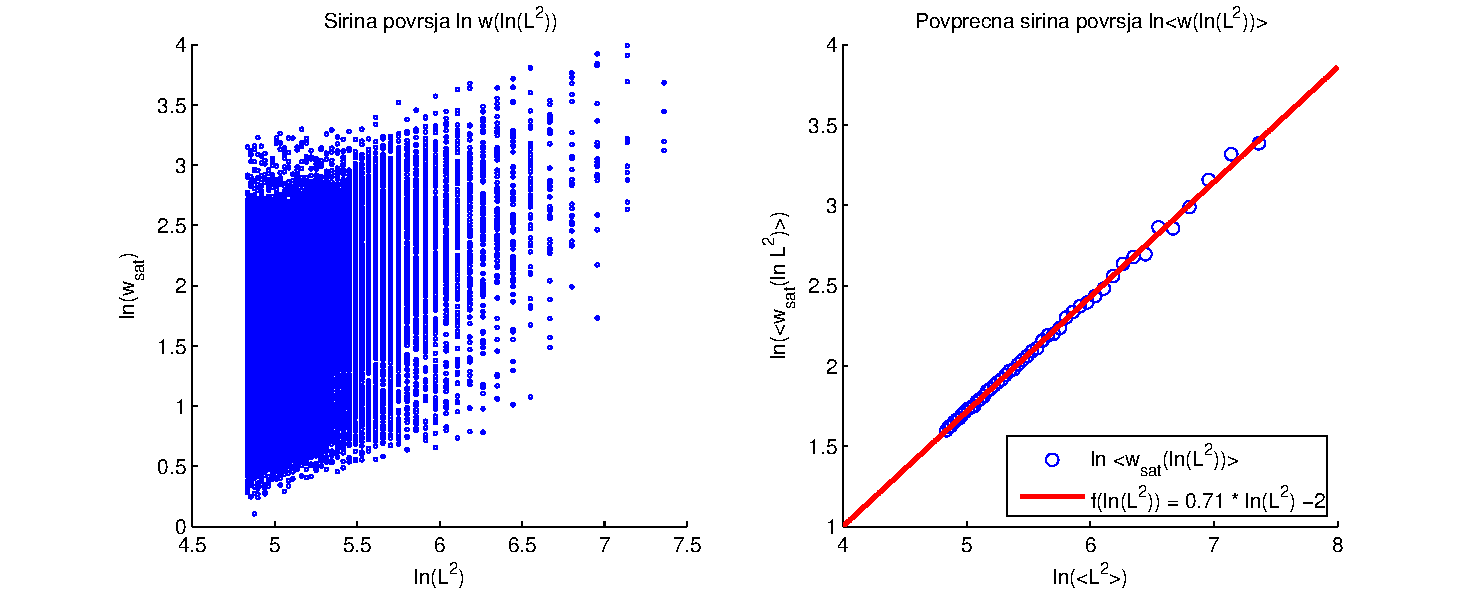
\includegraphics[width=1.1\textwidth]{slike/menisija-alfa-3d}
  \begin{equation} \alpha = \frac{\partial ( ln (w_{sat}) ) }{\partial ( ln (L^2) )} =  0,71 \pm 0.01 \end{equation}
\end{center}
\end{frame}

\subsection{Kardar-Parisi-Zhang}

\begin{frame}{Kardar-Parisi-Zhang}{Konstrukcija enačbe}
\begin{columns}
  \begin{column}{0.45\textwidth}
    \footnotesize
    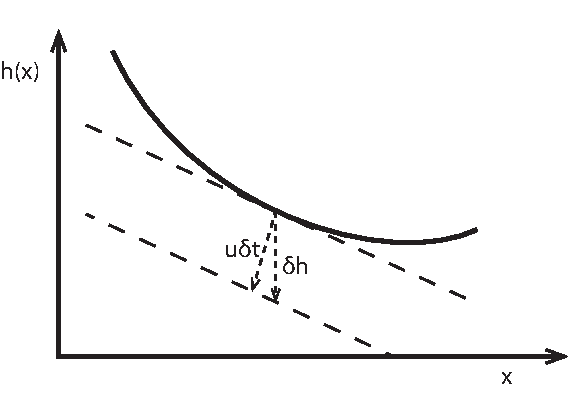
\includegraphics[width=1\textwidth]{slike/denudacija}
    \tiny{\\ Vir: Kardar-Parisi-Zhang, Dynamic Scaling of Growing Interfaces}
    \newline
    \newline
    Hitrost mikroskopske denudacije kamnine je obrnjena v kamnino:
    \begin{equation} \delta h = \sqrt{ (u \delta t)^2 + (u \delta t \nabla h)^2} \end{equation}   
    Če $|\nabla h| \ll 1$ dobimo: 
    \begin{equation} \frac{\partial h}{\partial t} \bigg|_{nelinearno} \simeq u + \frac{u}{2} (\nabla h)^2 + \dots \end{equation}
    
  \end{column}
  \begin{column}{0.55\textwidth}
    \tiny
    Privzamemo, da ima proces poleg stalne hitrosti denudacije kamnine $v$ še stohastično komponento $\eta(\mathbf{x},t)$:
    \begin{equation} \frac{\mathrm{d} h}{\mathrm{d} t} \bigg|_{denudacija} = v + \eta(\mathbf{x},t) \end{equation}
    Razpadanje kamnine je počasen proces, iz podlage odkrušeni kamni in prst se lahko premikajo, privzamemo v model še difuzijski člen:
\begin{equation} \frac{\mathrm{d} h}{\mathrm{d} t} \bigg|_{difuzija} = D \nabla^2 h \end{equation}
    \newline

    Pripravljene člene združimo v enačbo:
\begin{equation} \frac{\partial h}{\partial t} = \frac{\partial h}{\partial t} \bigg|_{denudacija} + \frac{\partial h}{\partial t} \bigg|_{difuzija} + \frac{\partial h}{\partial t} \bigg|_{nelinearno} \end{equation}
    Postavimo se premikajoč se koordinatni sistem s hitrostjo $v + u$ v smeri osi $h$ in dobimo Kardar-Parisi-Zhangovo enačbo:
    \begin{equation} \frac{\partial h}{\partial t} = D \nabla^2 h + \frac{u}{2} (\nabla h)^2 + \eta (\mathbf{x},t) \end{equation}
    \newline
    Kardar-Parisi-Zhang pokažejo, da ob pogoju da je $\eta(\mathbf{x},t)$ Gaussov šum velja:
    \begin{equation} \alpha = \frac{1}{2} \end{equation}
  \end{column}
\end{columns}

\end{frame}

\begin{frame}{Kardar-Parisi-Zhang}{Simulacija}
\begin{columns}
  \begin{column}{0.70\textwidth}
    \hspace*{-0.12\textwidth}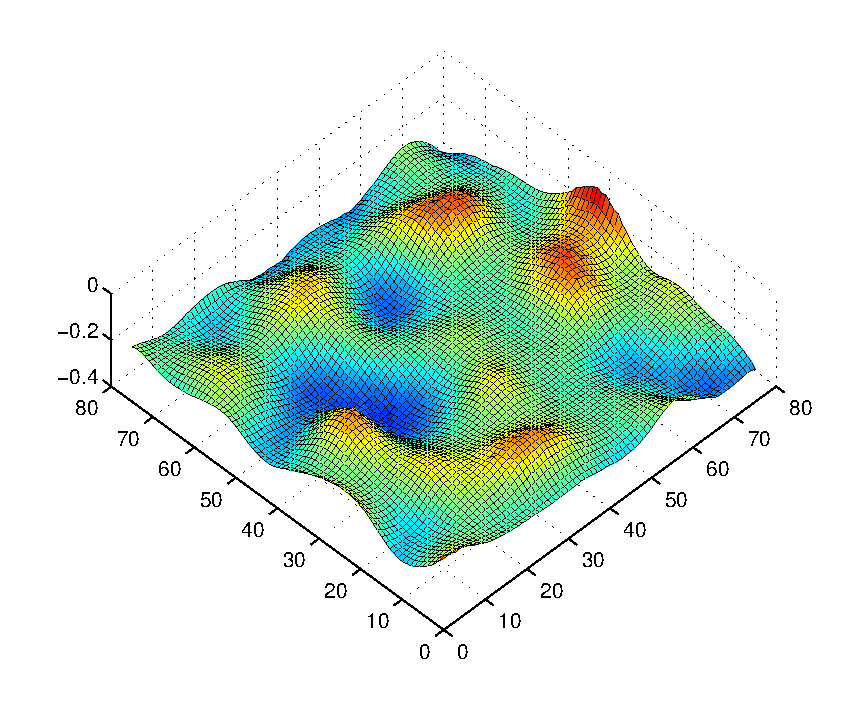
\includegraphics[width=1.25\textwidth]{slike/KPZ-numericno}
  \end{column}
  \tiny{}
  \hspace*{-0.18\textwidth}\begin{column}{0.5\textwidth}
    \begin{equation} h_{i+1} = h_i - dt (D \nabla^2 h_i + \frac{u}{2} (\boldsymbol\nabla h_i \cdot \boldsymbol\nabla h_i) + \eta (\mathbf{x},t)) \end{equation}
    \newline\newline\newline\newline\newline\newline\newline\newline\newline\newline\newline\newline\newline\newline
    \begin{itemize}
      \item
        Časovni korak $dt = 10^{-3}$
      \item
        Ponovimo $10^6$ krat
      \item
        Površje ni v ravnovesju.
      \item
       Hrapavost površja se ne spreminja več
    \end{itemize}

  \end{column}
\end{columns}
\end{frame}


\section{Modeliranje}

\subsection{Reakcijsko-difuzijski nastavki}

\begin{comment}
\begin{frame}{Reakcijsko-difuzijski nastavki}{Priraščanje površin ni primeren model za opis dinamike posameznih vrtač}
\begin{columns}
  \begin{column}{0.7\textwidth}
    \hspace*{-0.09\textwidth}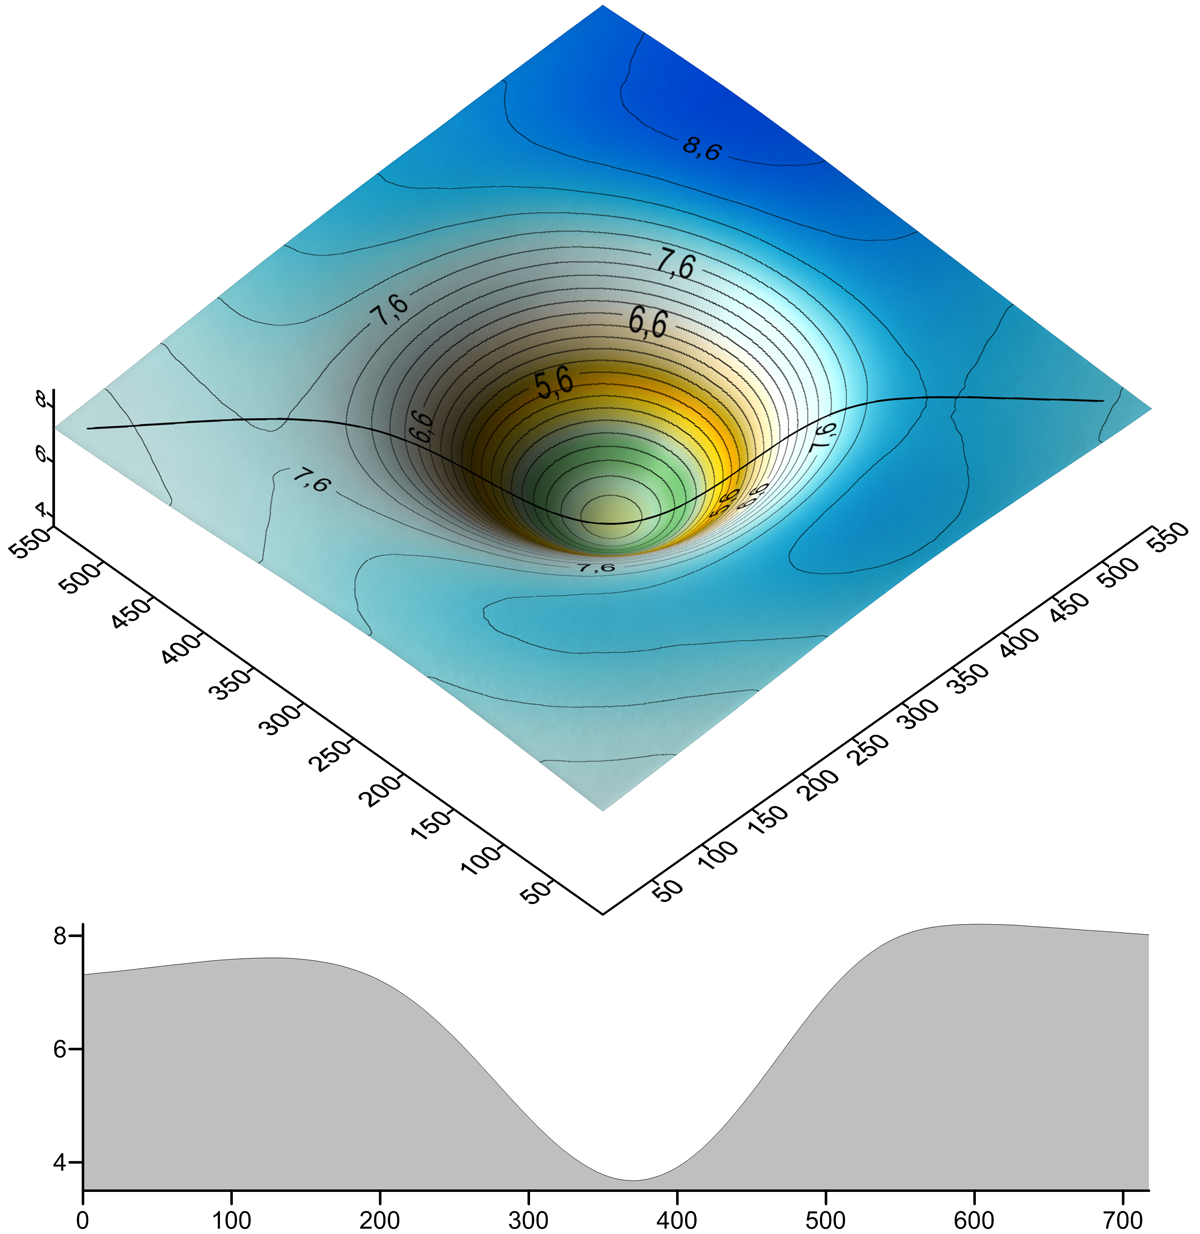
\includegraphics[width=\textwidth]{slike/menisija-vrtaca}
  \end{column}
  \begin{column}{0.3\textwidth}
    \hspace*{-0.3\textwidth}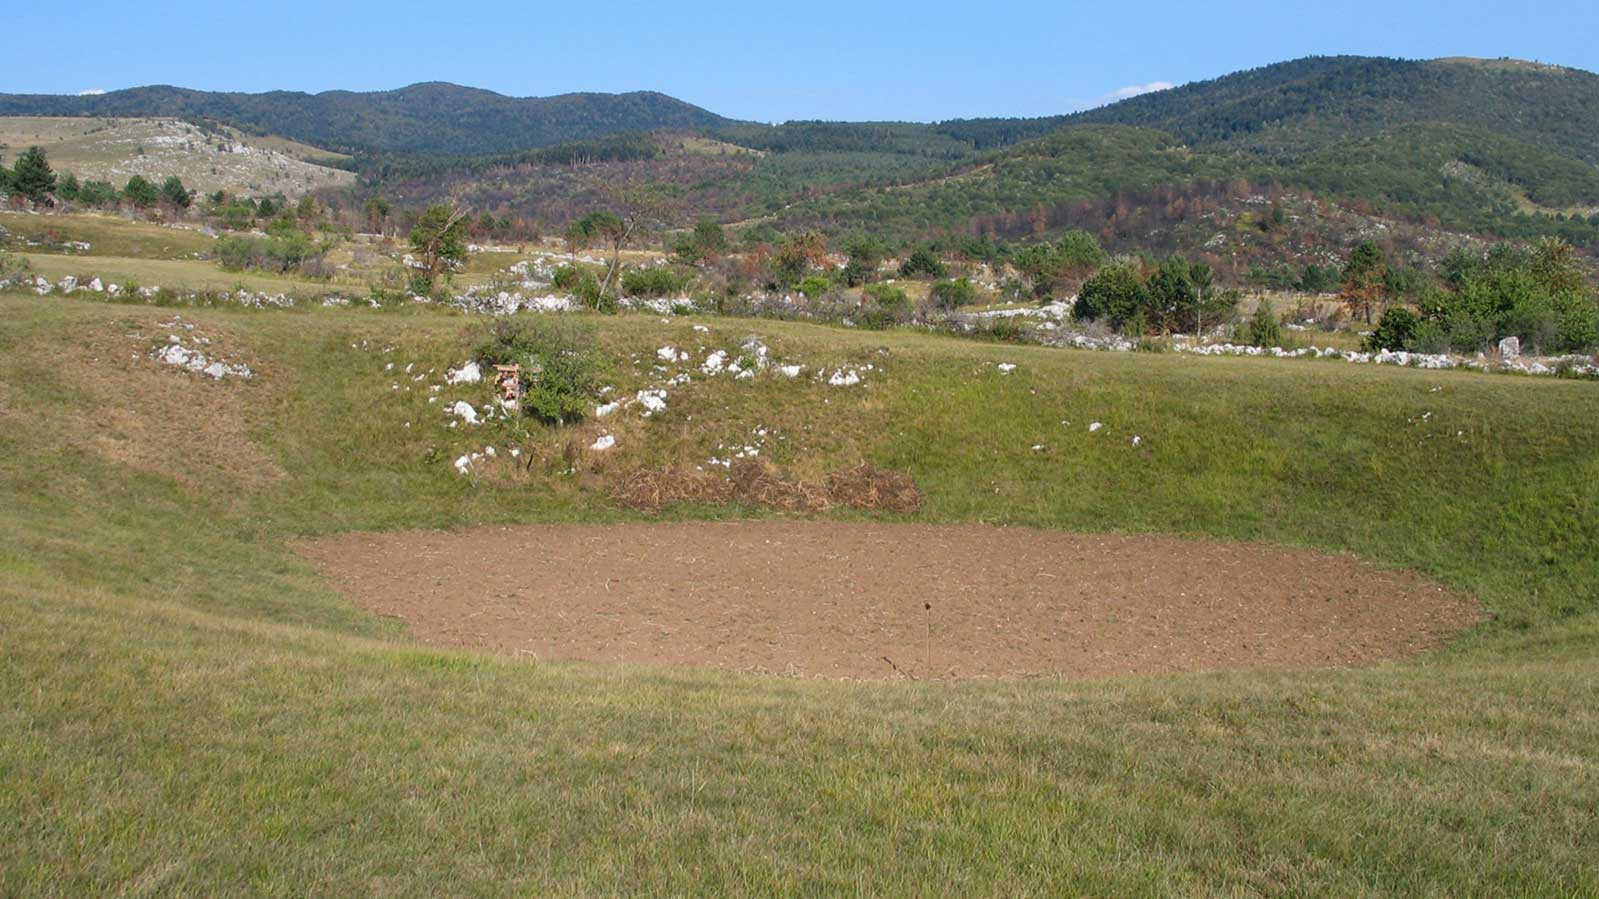
\includegraphics[width=1.4\textwidth]{slike/vrtaca}
    \tiny{\\ Vir: A.M.} \newline \newline
    \hspace*{-0.3\textwidth}\includegraphics[width=1.4\textwidth]{slike/verd}
    \tiny{\\ Vir: A.M}
  \end{column}
\end{columns}
\end{frame}
\end{comment}

\begin{frame}{Reakcijsko-difuzijski nastavki}{Prehod na determinističen opis}
\begin{block}{Stohastične enačbe}
  \begin{itemize}
  \item
    Kardar-Parisi-Zhang-ova rast površja nam ne da determinističnega modela rasti posamezne vrtače
  \item
    Možen je le izračun verjetnosti, da bomo pri danem površju dobili določeno končno površje
  \end{itemize}
\end{block}
\begin{block}{Reakcijsko-difuzijske enačbe}
  \begin{itemize}
  \item
    Zapišemo Kardar-Parisi-Zhangovo enačbo v obliko:
    \begin{equation} \frac{ \partial h}{ \partial t} = D \nabla^2 h + F(h), \end{equation}
    za člen $F(h)$ namesto linearne stohastične funkcije vstavimo različne fenomenološke modele rasti
  \item
    Najprej ločeno pogledamo deterministične nastavke
  \end{itemize}
\end{block}
\end{frame}


\begin{frame}{Reakcijsko-difuzijski nastavki}{Primer determinističnega nastavka: Omejena eksponentna rast}
\begin{block}{Model}
  Rast v času je odvisna od višine in razdalje do nosilne kapacitete. Odziv je odvisen od razdalje do nosilne kapacitete.
  \begin{equation} \frac{\partial h(t)}{\partial t} = a \cdot ( K - h(t) ) = a K - a h(t) \end{equation}
\end{block}
\begin{block}{Rešitev}
  \begin{equation} h(t) = K - (K - h_0) e^{-a t} \end{equation}
\end{block}
\begin{block}{Uporaba}
  Sistemi brez notranjih interakcij, kjer dinamiko poganjajo zunanji dejavniki. Na primer: širjenje informacij v družbi preko medijev.
\end{block}
\end{frame}

\begin{frame}{Reakcijsko-difuzijski nastavki}{Primer determinističnega nastavka: Omejena eksponentna rast}
\begin{center}
  \hspace*{-0.09\textwidth}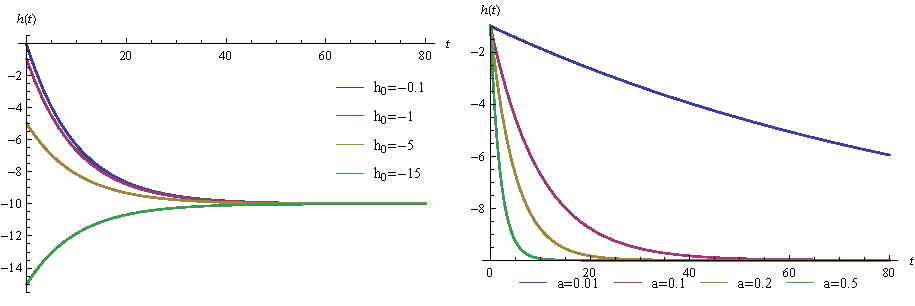
\includegraphics[width=1.2\textwidth]{slike/omejena-eksponentna-rast}
  \footnotesize
\begin{columns}
  \begin{column}{0.5\textwidth}
  \[ K = -10 \]
  \[ a = 0.1 \]
  \end{column}
  \begin{column}{0.5\textwidth}
  \[ K = -10 \]
  \[ h_0 =-1 \]
  \end{column}
\end{columns}
\end{center}
\end{frame}


\begin{frame}{Reakcijsko-difuzijski nastavki}{Primer determinističnega nastavka: Logistična rast}
\begin{block}{Model}
  Rast v času je odvisna od višine in razdalje do nosilne kapacitete. \\
  Odziv je manj skokovit kot pri omejeni eksponentni rasti.
  \begin{equation} \frac{\partial h(t)}{\partial t} = a \cdot \left( 1 - \frac{h(t)}{K} \right) h(t) \end{equation}
\end{block}
\begin{block}{Rešitev}
  \begin{equation} h(t) = \frac{h_0 K e^{a t}}{K + h_0 (e^{a t}-1)} \end{equation}
\end{block}
\begin{block}{Uporaba}
  Sistemi ki jih omejuje nosilna kapaciteta okolja, na primer: živalske populacije, rast tumorjev.
\end{block}
\end{frame}

\begin{frame}{Reakcijsko-difuzijski nastavki}{Primer determinističnega nastavka: Logistična rast}
\begin{center}
  \hspace*{-0.09\textwidth}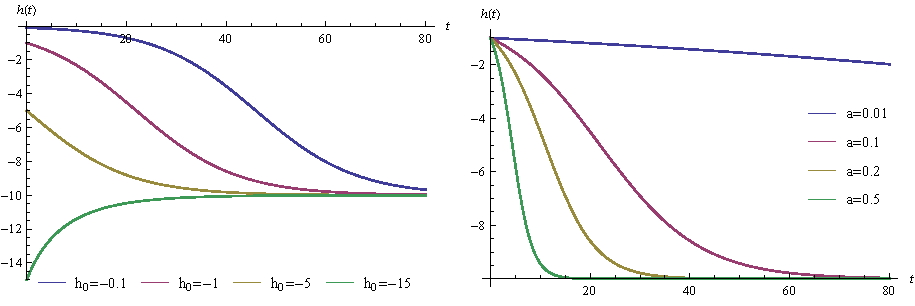
\includegraphics[width=1.2\textwidth]{slike/logisticna-rast}
  \footnotesize
\begin{columns}
  \begin{column}{0.5\textwidth}
  \[ K = 10 \]
  \[ a = 0.1 \]
  \end{column}
  \begin{column}{0.5\textwidth}
  \[ K = 10 \]
  \[ h_0 = 0.1 \]
  \end{column}
\end{columns}
\end{center}
\end{frame}


\subsection{Reakcijsko-difuzijske enačbe}

\begin{frame}{Reakcijsko-difuzijske enačbe}{Dodamo difuzijski člen}

\begin{block}{Dinamični nastavki}
  \begin{itemize}
  \item
    Nam dajo modele rasti
  \item
    Nastavke rasti izberemo tako, da so smiselni za rast vrtače
  \end{itemize}
\end{block}
\begin{block}{Reakcijsko-difuzijske enačbe}
  \begin{itemize}
  \item
    So oblike: \begin{equation}  \frac{ \partial h(t,x) }{ \partial t} = - \nabla j(t,x) + F( h(t) )= D \Delta h(t,x) + F( h(t) ) \end{equation}
  \item
    Izberemo smiselne robne pogoje, rešujemo numerično v dveh dimenzijah in času
  \end{itemize}
\end{block}
\end{frame}


\begin{frame}{Reakcijsko-difuzijske enačbe}{Primer: Omejena eksponentna rast}
\begin{block}{Model}
 Omejena eksponentna rast:
  \begin{equation} \frac{ \partial h(\mathbf{x},t) }{ \partial t} = D \frac{\partial^2}{\partial \mathbf{x}^2} h(\mathbf{x},t) + a \cdot (K - h(\mathbf{x},t)) \end{equation} 
\end{block}
\begin{block}{Robni pogoji}
    \begin{equation}
      \begin{aligned}
        h(\mathbf{x},0) =  - e^{-\mathbf{x}^2}, \mathbf{x} \in D \\
        h(\mathbf{x},t) = 0, \mathbf{x} \in \partial D \\
        \mathbf{n} \cdot \boldsymbol \nabla h(\mathbf{x},t) = 0, \mathbf{x} \in \partial D,
      \end{aligned}
    \end{equation}
\end{block}
\end{frame}

\begin{frame}{Reakcijsko-difuzijske enačbe}{Primer:  Omejena eksponentna rast}
\begin{columns}
  \begin{column}{0.8\textwidth}
    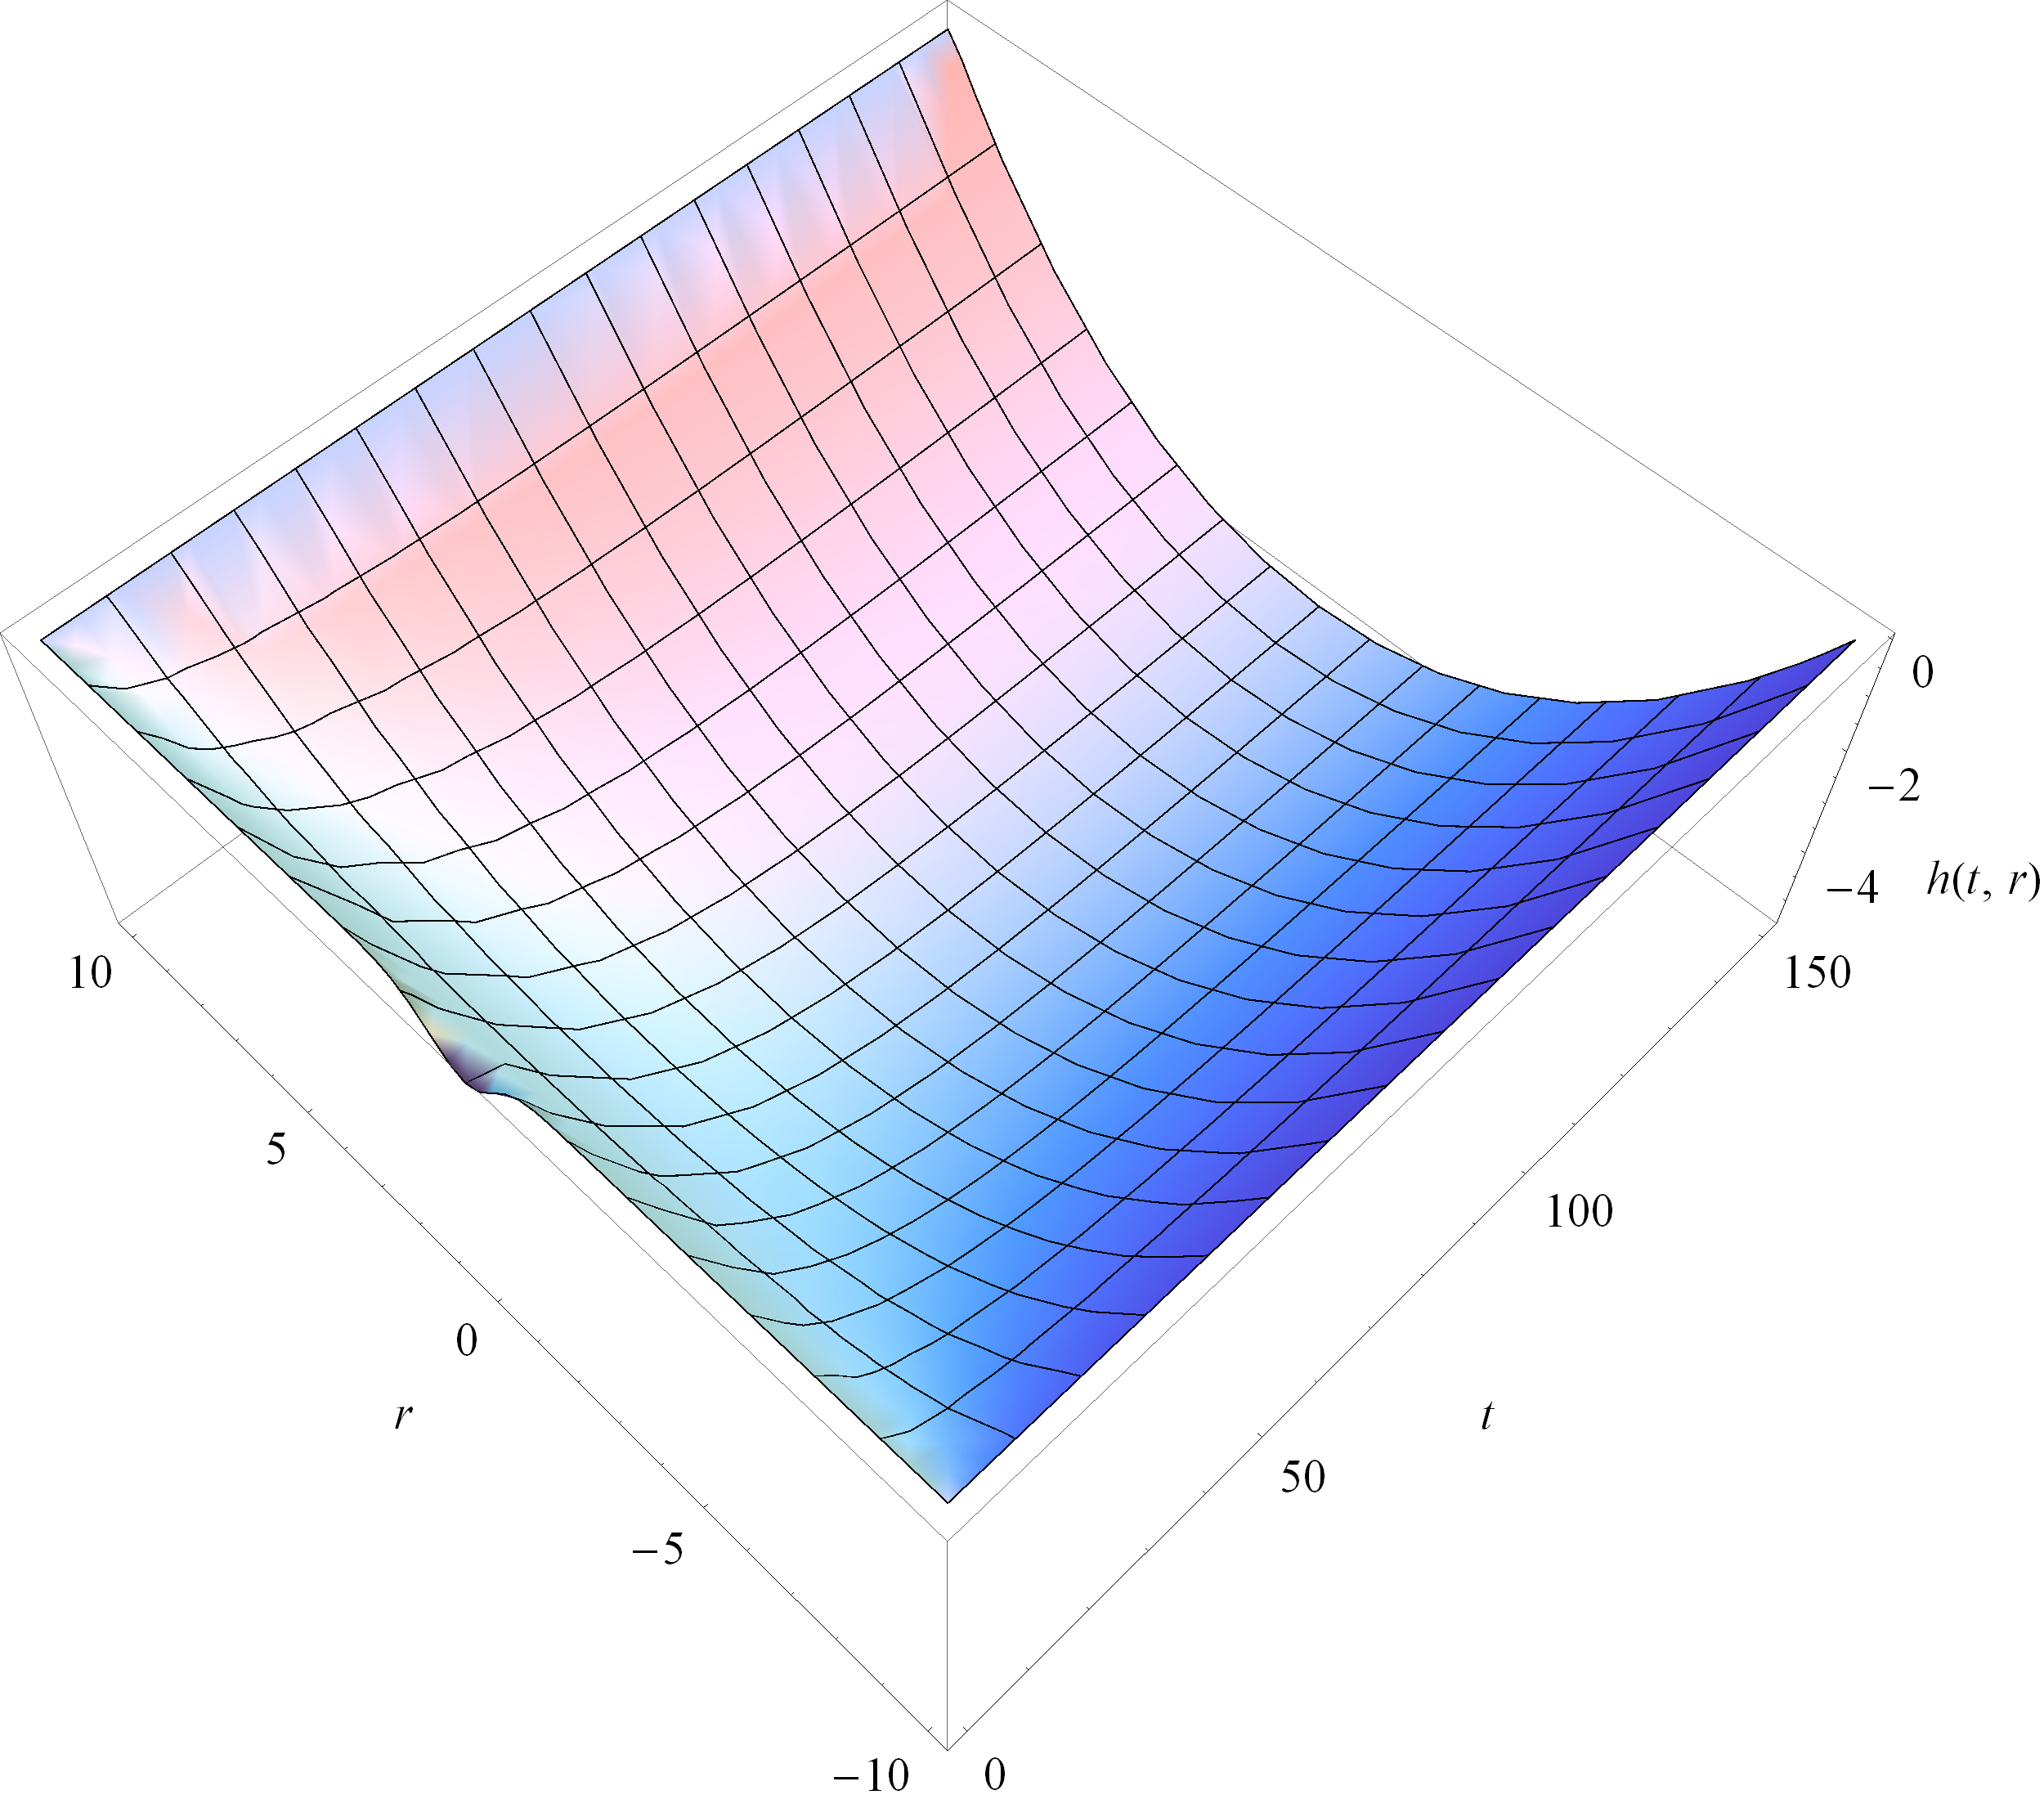
\includegraphics[width=1.05\textwidth]{slike/difuzija-omejena-eksponentna-rast2.png}
  \end{column}
  \begin{column}{0.3\textwidth}
    \footnotesize
    \[ D = 1 \]
    \[ a = \frac{1}{50} \]
    \[ K = -10 \]
  \end{column}
\end{columns}
\end{frame}


\begin{frame}{Reakcijsko-difuzijske enačbe}{Primer: Logistična rast}
\begin{block}{Model}
  Logistična rast z difuzijo ali Fisher-Kolmogorov-a enačba:
  \begin{equation}  \frac{ \partial h(\mathbf{x},t) }{ \partial t} = D \frac{\partial^2}{\partial \mathbf{x}^2} h(\mathbf{x},t) + a \cdot h(\mathbf{x},t) \cdot (1 - \frac{h(\mathbf{x},t)}{K}) \end{equation} 
\end{block}
\begin{block}{Robni pogoji}
    \begin{equation}
      \begin{aligned}
        h(\mathbf{x},0) =  - e^{-\mathbf{x}^2}, \mathbf{x} \in D \\
        h(\mathbf{x},t) = 0, \mathbf{x} \in \partial D \\
        \mathbf{n} \cdot \boldsymbol \nabla h(\mathbf{x},t) = 0, \mathbf{x} \in \partial D,
      \end{aligned}
    \end{equation}
\end{block}
\end{frame}

\begin{frame}{Reakcijsko-difuzijske enačbe}{Primer: Logistična rast}
\begin{columns}
  \begin{column}{0.8\textwidth}
    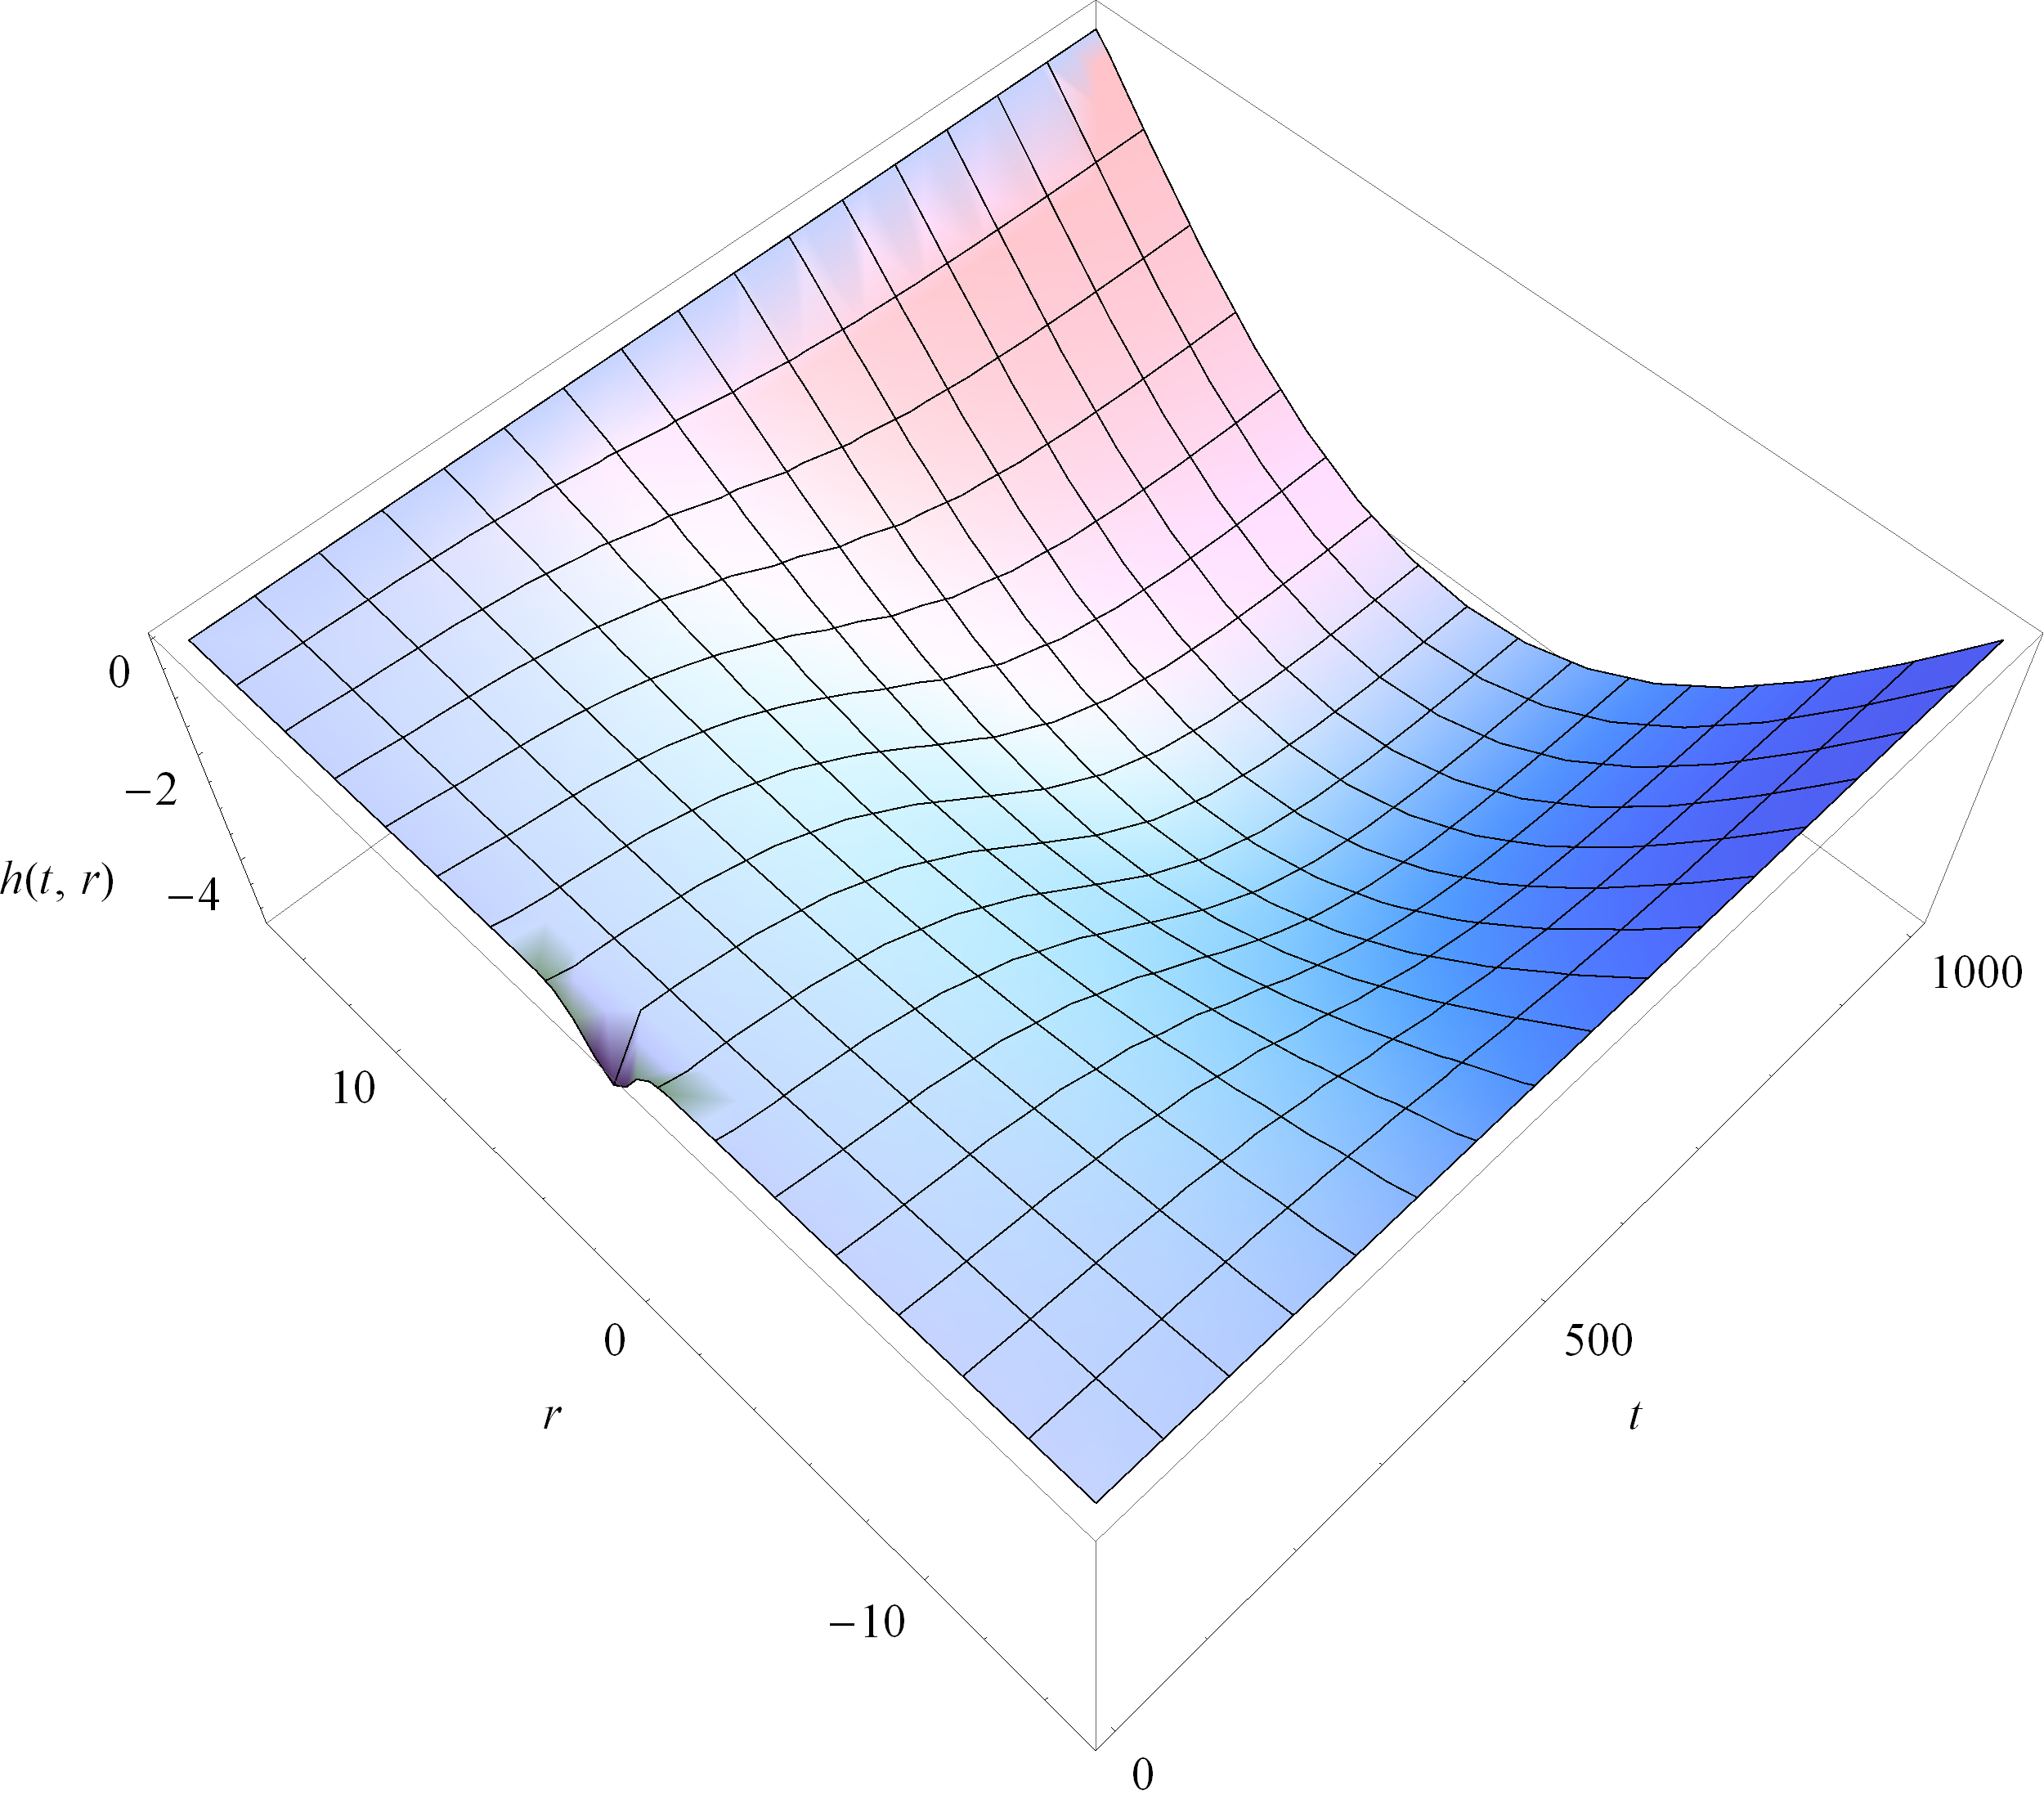
\includegraphics[width=1.05\textwidth]{slike/difuzija-logisticna-rast2.png}
  \end{column}
  \begin{column}{0.3\textwidth}
    \footnotesize
    \[ D = 1 \]
    \[ a = \frac{1}{50} \]
    \[ K = -10 \]
  \end{column}
\end{columns}
\end{frame}


% Placing a * after \section means it will not show in the
% outline or table of contents.
\section*{Zaključek}

\begin{frame}{Povzetek}
  \begin{itemize}
  \item<1->
    Segmentacija in analiza vrtač na digitalnem reliefu je relativno enostavna naloga
  \item<2->
    Vrtače so približno Gaussove oblike
  \item<3->
    Kardar-Parisi-Zhang-ova rast površin napove podobno hrapavost, kot jo opazimo v Menišiji
  \item<4->
    Izbira fizikalnega modela je zaradi pomanjkanja informacij o časovni dinamiki težka, natančnejši geološki študij dinamike reliefa bi bil v pomoč
  \item<5->
    Najbolj pravilen model se zdi Fisher-Kolmogorova enačba zaradi:
    \begin{itemize}
      \item<6->
        časovnega razvoja oblike profila
      \item<7->
        končne oblike pobočja profila
    \end{itemize}
  \end{itemize}
\end{frame}


\begin{comment}
\appendix
\section<presentation>*{\appendixname}
\subsection<presentation>*{Bibliografija}

\begin{frame}[allowframebreaks]
  \frametitle<presentation>{Bibliografija}
    
  \begin{thebibliography}{10}
    
  \beamertemplatebookbibitems
  % Start with overview books.

  \bibitem{Author1990}
    A.~Author.
    \newblock {\em Handbook of Everything}.
    \newblock Some Press, 1990.
 
    
  \beamertemplatearticlebibitems
  % Followed by interesting articles. Keep the list short. 

  \bibitem{Someone2000}
    S.~Someone.
    \newblock On this and that.
    \newblock {\em Journal of This and That}, 2(1):50--100,
    2000.
  \end{thebibliography}
\end{frame}

\end{comment}

\end{document}


